%%%%%%%%%%%%%%%%%%%%%%% file template.tex %%%%%%%%%%%%%%%%%%%%%%%%%
%
% This is a general template file for the LaTeX package SVJour3
% for Springer journals.          Springer Heidelberg 2010/09/16
%
% Copy it to a new file with a new name and use it as the basis
% for your article. Delete % signs as needed.
%
% This template includes a few options for different layouts and
% content for various journals. Please consult a previous issue of
% your journal as needed.
%
%%%%%%%%%%%%%%%%%%%%%%%%%%%%%%%%%%%%%%%%%%%%%%%%%%%%%%%%%%%%%%%%%%%
%
% First comes an example EPS file -- just ignore it and 
% proceed on the \documentclass line
% your LaTeX will extract the file if required
\begin{filecontents*}{example.eps}
%!PS-Adobe-3.0 EPSF-3.0
%%BoundingBox: 19 19 221 221
%%CreationDate: Mon Sep 29 1997
%%Creator: programmed by hand (JK)
%%EndComments
gsave
newpath
  20 20 moveto
  20 220 lineto
  220 220 lineto
  220 20 lineto
closepath
2 setlinewidth
gsave
  .4 setgray fill
grestore
stroke
grestore
\end{filecontents*}
%
\RequirePackage{fix-cm}
%
%\documentclass{svjour3}                     % onecolumn (standard format)
%\documentclass[smallcondensed]{svjour3}     % onecolumn (ditto)
%\documentclass[smallextended]{svjour3}       % onecolumn (second format)
\documentclass[twocolumn]{svjour3}          % twocolumn
%
\smartqed  % flush right qed marks, e.g. at end of proof

%\usepackage{subfig}
%\usepackage{subcaption}

\usepackage{graphicx}
\usepackage{amssymb}
\usepackage{amsmath}
%\usepackage{bm}
\usepackage{amsfonts}
\usepackage{array}
\usepackage{multirow}
\usepackage{flushend}
\usepackage[numbers, sort&compress]{natbib}
\usepackage{txfonts}
\usepackage{graphicx}
\usepackage{epstopdf}

%\usepackage{fontspec}
%\captionsetup{compatibility=false}
%\usepackage[caption=false]{subfig}
%\usepackage[caption=false]{subfig}
\usepackage{comment}
\usepackage{amsmath}
\usepackage{amsfonts}
\usepackage{graphicx}
%\usepackage{epstopdf}
\usepackage{xcolor}
\renewcommand{\vec}[1]{\boldsymbol{#1}}



%try deal with overhull
%\usepackage[textwidth=14.5cm]{geometry}
%\usepackage{blindtext}
%\parindent=0pt
% try deal with overhull

\usepackage[hidelinks]{hyperref}
\usepackage{tikz}
\usetikzlibrary{calc}
\usetikzlibrary{decorations.text}
\usepackage{mathptmx} % use Times fonts if available on your TeX system
\newcommand{\ud}{\mathrm{d}}
\newcommand{\uT}{\mathrm{T}}
\newcommand{\vect}[1]{\boldsymbol{\mathbf{#1}}}
\makeatletter
\def\hlinewd#1{%
\noalign{\ifnum0=`}\fi\hrule \@height #1 %
\futurelet\reserved@a\@xhline}
\makeatother
%
% insert here the call for the packages your document requires
%\usepackage{latexsym}
% etc.
%
% please place your own definitions here and don't use \def but
% \newcommand{}{}
%
% Insert the name of "your journal" with
% \journalname{myjournal}
%
% \input{deffile.tex}
\begin{document}
\begin{sloppypar}
\title{A noval guidance control of a thruster-assisted position mooring system with model-based reinforcement learning
	%Optimal Setpoint Learning of a Thruster-assisted Position Mooring System with Model-based Acceleration
	%\thanks{Grants or other notes
	%about the article that should go on the front page should be
	%placed here. General acknowledgments should be placed at the end of the article.}
}
%\subtitle{Do you have a subtitle?\\ If so, write it here}

%\titlerunning{}        % if too long for running head

\author{Xu Jiang1 \and
	Lei Wang     \and
	Shangyu Yu     \and
	Huacheng He	 \and
	Te Yu
}

%\authorrunning{Short form of author list} % if too long for running head

\institute{Lei Wang\\
	\email{wanglei@sjtu.edu.cn}\\ \at
	State Key Laboratory of Ocean Engineering, Shanghai Jiao Tong University, Shanghai, China 200240 \\
	Collaborative Innovation Center for Advanced Ship and Deep-Sea Exploration, Shanghai, China 200240 \\
	School of Naval Architecture, Ocean and Civil Engineering, Shanghai Jiao Tong University, Shanghai, China 200240 
	%              Tel.: +123-45-678910\\
	%              Fax: +123-45-678910\\
	%             \emph{Present address:} of F. Author  %  if needed
}

\date{Received: date / Accepted: date}
% The correct dates will be entered by the editor


\maketitle
\begin{abstract}
{\it Thruster-assisted position mooring (PM) systems use both mooring lines and thrusters for station keeping of marine structures in ocean environments. In order to operate in an energy-efficient manner in moderate sea conditions, setpoints need to be appropriately chosen for the setpoint controller, so that the mooring system counteracts main environmental loads, while the thrusters reduce oscillatory motions of the marine structure. Reinforcement learning (RL) is a powerful and effective approach to designing decision making agents for setpoint selection. We propose a model-based reinforcement learning method which interplays direct and indirect learning to update Q-function. The reward function of the world model is approximated by support vector regression. Extensive simulation results indicate that the proposed RL agents can successfully identify the optimal setpoints through continuous planning, acting and learning in an unknown and stochastic environment, and the model-based approach accelerates the learning speed of the decision making agent.}
	
\keywords{thruster-assisted position mooring \and optimal setpoint \and reinforcement learning \and Model-based Q-learning \and neural network}
	% \PACS{PACS code1 \and PACS code2 \and more}
	% \subclass{MSC code1 \and MSC code2 \and more}
\end{abstract}

\section{INTRODUCTION}
\label{sec:intro}

For offshore exploitation and exploration in intermediate water depths, mooring vessels with thruster assistence (positon mooring-PM) are often the most cost-effective and feasible solution to stationkeeping operation compared with fixed platforms and dynamic positioned (DP) vessels\cite{nguyen2009switching}. The reason is that a PM system is uaually regarded as the combination of the mooring and DP system. And the mooring system provides effective passive control to compensate the mean environment loads at the intermediate water depths, while the DP systems can perform active control to reduce structure offset and keep the mooring line tensions within a safety limit in order to prevent line breakage. And PM systems have been commercially available since the 1980s and generally becomes a flexible choice for drilling and oil exploitation on the marginal fields\cite{sorensen2011survey}.


%A thruster-assisted position mooring system, usually referred to as PM system, consists of mooring lines and thrusters to maintain the position and heading of a marine structure. PM systems have been commercially available since the 1980s and generally becomes a flexible choice for drilling and oil exploitation on the marginal fields\cite{sorensen2011survey}. The main contribution of the mooring lines is to compensate the mean environmental loads, while the thrusters provide forces to reduce structure offset and keep the mooring line tension within a safety limit in order to prevent line breakage.  Compared with dynamic positioning (DP) system, PM system provides a more cost-effective solution for station-keeping in many deep-water operations. 

There have been extensive studies on control strategies for DP and PM systems. \cite{aarset1998nonlinear} proposed the nonlinear feedback linearization and back-stepping control for DP.  In the work of \cite{fossen1999passive}, a passive nonlinear observer with adaptive wave filtering is proposed, which reduces the number of tuning parameters. Further, \cite{tannuri2010dynamic} presented to use nonlinear sliding mode control for DP and couducted corresponding experiments. In terms of PM systems, \cite{aalbers1996hydrodynamic} conducted model tests for a PM FPSO in a wide range of water depths. A PID controller was implemented in the tests to keep the center of the vessel turret at a reference position, and the heading into the waves. \cite{strand1998design} presented a mathematical model of a PM vessel, and defined four control modes of operation for surge, sway and yaw, including manual, damping, setpoint and tracking control. Simulation results showed that heading setpoint control was crucial for turret-anchored ships, and damping control of surge and sway reduced oscillatory motions, which are induced by slowly varying environmental loads. \cite{aamo1999controlling} used the finite element method to model the dynamics of the mooring lines, and proposed the design of a dynamic line tensioning controller to minimize the energy consumption of thrusters by changing the length of mooring lines. \cite{sorensen1999thruster} designed a nonlinear passive observer for PM ships, and presented the results of a full-scale test with a turret-anchored FPSO. \cite{wichers1999benefits} performed numerical simulations of a DP assisted turret moored FPSO to show that a light mooring system with a DP system is equivalent to withstand the same survival condition as a heavy passive mooring system. \cite{ryu2003coupled} conducted a fully coupled hull/mooring/riser dynamic analysis of a thruster-assisted turret-moored FPSO. The simulation results showed that the vessel's horizontal-plane response and the tensions of mooring lines and the riser were greatly reduced by the PM system. 

As the DP technology became more mature, guidance systems are taken into consideration for satisfying the integration of operational requirements and the performance of vessel control systems.  \cite{sorensen2001optimal} represented the concept of optimal setpoint chasing for deep-water drilling. Further,  \cite{leira2006structural} proposed to use structural reliability criteria of the drilling risers for the setpoint chasing. Considering the automatic switching between several controllers for a PM system when the environmental condition changes, \cite{nguyen2009switching} proposed to integrate the controllers into a supervisory control system, and employed both mean disturbance loads and wave peak frequency as the parameters to switch between controllers. By integrating an appropriate bank of controllers and models at the pant control level into a hybrid DP system, such supervisory-switched methodology is able to operate in varying environmental conditions. \cite{ren2015supervisory} developed a fault-tolerant control strategy for a PM vessel based on supervisory control method as well. A bank of passive observers were implemented to detect mooring line breakages and generate monitoring signals for the supervisor to select the most suitable controller.

When a PM system is in setpoint control mode, appropriate selection of setpoints is crucial for both the safety and performance of the PM system. \cite{nguyen2010control} proposed a control strategy using mooring line tensioning and heading control by thrusters to reduce riser end angle deviations. The optimal setpoint was determined using the finite element model of the riser. Simulations and experiments verified that vessel offsets and riser end angle could be reduced by applying thruster actions and actively changing the mooring line length. \cite{fang2013position} proposed a setpoint chasing approach for a PM system, which calculated the optimal setpoint based on a structural reliability criterion in order to keep all mooring lines at a specified reliability level. \cite{nguyen2009setpoint} proposed a setpoint chasing algorithm for PM systems. The low-frequency position of the vessel was chosen as the setpoint for thruster control in moderate sea conditions where the mooring lines compensate the mean environmental loads while thruster actions provided additional damping and restoring forces. In extreme conditions, the simulations and experiments suggested a position closer to the field zero point than the equilibrium point as the setpoint in order to reduce the mooring line tensions and vessel offset. \cite{bjorno2017modeling} tested the setpoint chasing algorithm on a thruster-assisted turret-moored drillship in model tests. The experiments showed that the control algorithm reduced thruster usage and maximized the utilization of mooring system. \cite{wang2016numerical} undertook both numerical and experimental studies on the influence of setpoint positions on the performance of a PM system. The results illustrated that the equilibrium point of the mooring system is the optimal setpoint in terms of positioning accuracy and power consumption of the thrusters. 

In recent years, with the heated discussion of machine learning techniques especially reinforcement learning,many researchers have been searching the potential of using these techniques for industrial assets. Reinforcement learning is a maturing field in artificial intelligence, where a significant portion of the research is concerned with approaches  in virtual environments \cite{sutton1999reinforcement}. During the training process, the algorithm learns how the transition function changes and estimates a state-value function $V$ or state-action value $Q$ that represent the value of being in the current state.\cite{anderlini2018reactive} adopted a model-free Q-learning method, a powerful reinforcement learning technique, to predict the wave energy distribution for energy collection.\cite{nagabandi2018neural} proposed a model-based reinforcement learning algorithm which combined a  medium-size neural network model with model predictive control. The simulation results demonstrated that this model-based approach can quickly become competent for a given task. However, this method might be inapplicable with high-dimensional actions spaces. \cite{magalhaes2018reinforcement} developed a bio-mimetic underwater vehicle controller with Q-learning. The control policy was first trained by a simulator, then the updated neural network parameters were transferred to a real vehicle for validation. Recently, \cite{woo2019deep} designed a path following algorithm for unmanned surface vehicle (USV) with a deep deterministic policy gradient (DDPG) approach. Model tests demonstrated that by interacting with the environment, the USV learned the optimal policy successfully.

The objective of this paper is to develop an automated intelligent support agent which provides optimal setpoints for low-level setpoint controllers to follow. The novel decision-making strategy is based on both model-free and model-based reinforcement learning, goal-oriented machine learning tools with which the decision maker learns a policy from scratch to maximize long-term rewards through interactions with the unknown environment. By implementing the intelligent setpoint control strategies, the utilization of the mooring system is maximized to compensate the mean environmental loads, while the thruster actions reduce the oscillatory motion of the platform around the optimal setpoint.

The rest of the paper is organized as follows: the mathematical dynamics of a PM floating structure is introduced in section 2. In section 3, the plant control design of the PM system is addressed. Time-domain simulations are performed to demonstrate the control performances of the PM system in both damping and setpoint control modes. The automated intelligent support agent for generating optimal setpoints is then presented in section 4. The decision-making strategy based on reinforcement learning is adopted, and numerical experiments are conducted for validation and discussion. Finally, the main conclusions are presented in section 5.

\section{MATHEMATICAL MODELING OF A PM FLOATING STRUCTURE}
\label{MATHEMATICAL MODELING}
%%%%%%%%%%%%%%%%%%%%%%%%%%%%%%%%%%%%%%%%
As shown in Fig.~\ref{fig:coordinate}, A global coordinate system is defined as $(X_G, Y_G, Z_G)$ with origin $O_G$. For a PM system, the origin of the global coordinate system is usually the field zero point of the mooring system. The 6 degree-of-freedom dynamics of a semi-submersible platform in the time domain can be described using the Cummins equations \cite{cao2010effects}, which are defined in the local coordinate system $(X, Y, Z)$ fixed with respect to the mean position of the semi-submersible platform:

\begin{figure}[htbp]
	\centering
	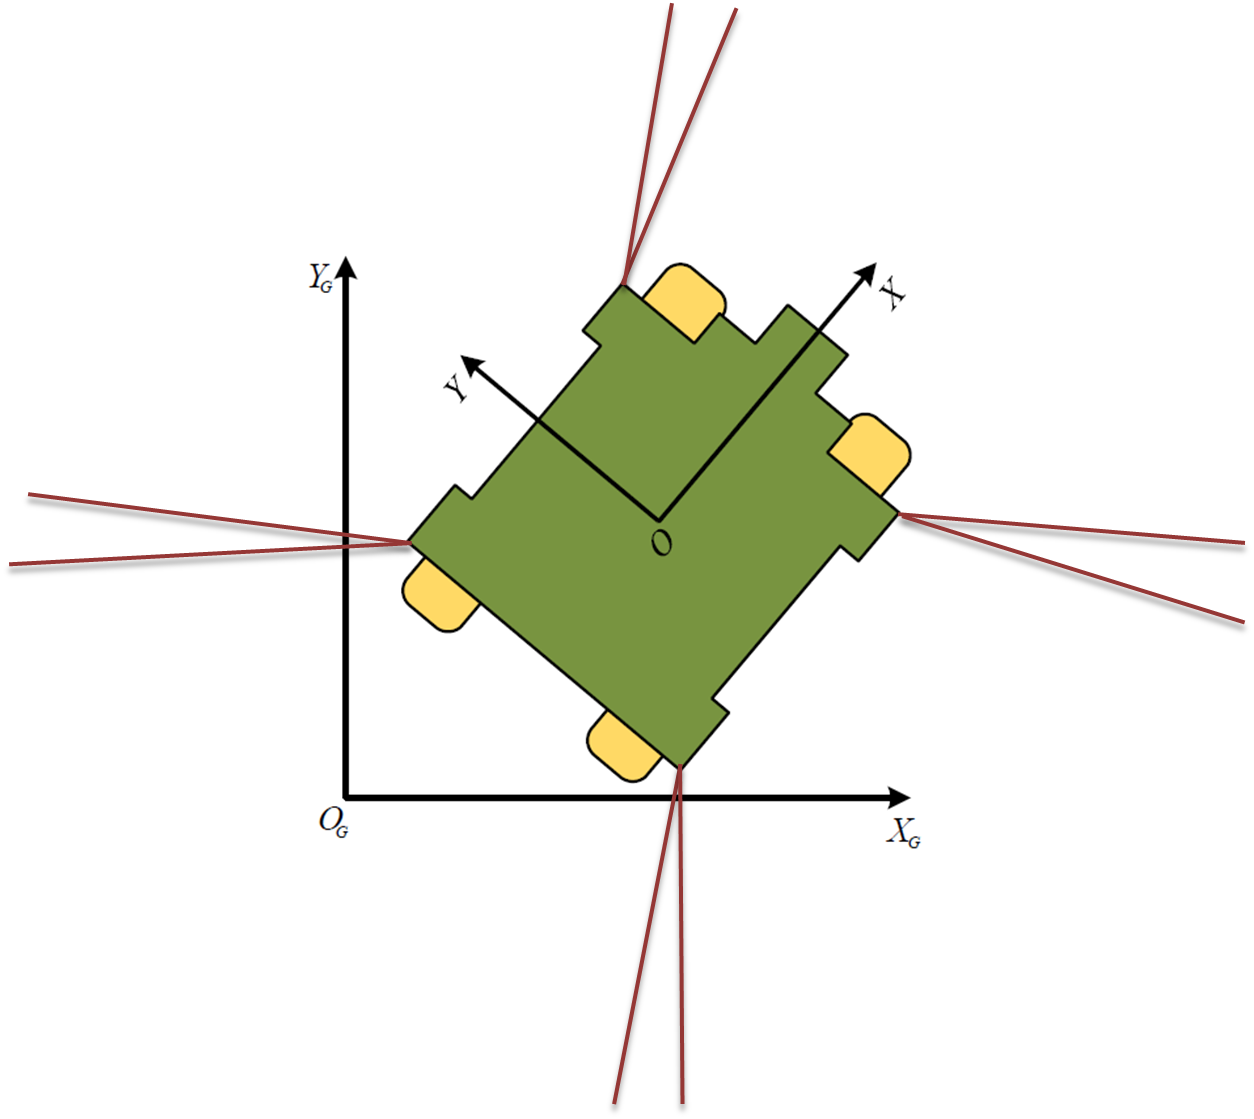
\includegraphics[width=3.0in]{Images/coordinate_new.png}
	\caption{The global and local coordinate systems.}
	\label{fig:coordinate}
\end{figure}

\begin{equation}
(\vec{M}_{RB} + \vec{A}(\infty))\ddot{\vec{p}} + \int_{0}^{t}\vec{K}(t-\tau)\dot{\vec{p}}(\tau)\mathrm{d}\tau + \vec{C}\vec{p} = \vec{F}(t)
\end{equation}

\noindent where $\vec{M}_{RB}, \vec{A}(\infty), \vec{K(t)}, \vec{C} \in\mathbb{R}^{6\times6}$ are respectively the mass matrix of the platform, the constant infinite-frequency added mass matrix, the matrix of retardation function, and the matrix of hydrostatic restoring forces, and $\vec{p}$ represents the displacements in the six modes of response. Given the frequency-dependent added mass $\vec{A}(\omega)$ and damping matrices $\vec{B}(\omega)$, we have:

\begin{align}
\vec{K}(t) &= \frac{2}{\pi}\int_{0}^{\infty}\vec{B}(\omega)\cos(\omega t)\mathrm{d}\omega \\
\vec{A}(\infty) &= \vec{A}(\omega) + \frac{1}{\omega}\int_{0}^{\infty}\vec{K}(\tau)\sin(\omega \tau)\mathrm{d}\tau
\end{align}

The term $\vec{F}(t)$ takes into account other time-varying loads, such as wave loads, viscous damping forces, wind and current  loads, as well as mooring and thruster forces. The wave load effect on the platform includes both first-order wave excitation forces and second-order wave drift forces, which can be obtained using the force response amplitude operators (RAOs) and quadratic transfer functions (QTFs), respectively.

Due to the environmental loads, both the platform motion and mooring line tension have a mean static component plus wave frequency and low frequency dynamic components. The responses can be estimated in the frequency domain and time domain \cite{gao2009mooring}. There are mainly two dominating treatments of the mooring line dynamics in the time domain: the slender rod model and the lumped mass model. In the lumped mass method, mooring line is spatial discretized into lumped mass nodes which are connected with massless springs. Discretization in this way simplifies the mathematical model and provides numerical efficiency \cite{chai2002three, low2006time, xiong2016dynamics}. Furthermore, each item in the lumped mass model has a clear physical meaning, which facilitates the understanding and programming.

\section{PLANT CONTROL DESIGN OF PM SYSTEMS}

The design of the PM control system is divided into two levels: low-level plant control of the semi-submersible platform, and high-level decision making of the optimal setpoint for the low-level controller. In this section, the designs of the low-level feedback controllers are presented.

The PM system usually has several automatic control modes for operation, such as damping and setpoint control. The position and heading angle of the semi-submersible platform are measured in the global coordinate system, which contains high-frequency motions induced by the first-order wave excitation forces. Therefore, an observer is necessary to estimate low-frequency position and velocity of the platform for the feedback controllers. A thrust allocation algorithm is also introduced to allocate commanded forces among the azimuth thrusters of the platform.

\subsection{Controller Design}

When designing the low-level controllers for the PM system, it is advantageous to present the platform dynamics in a polar coordinate, so that weathervaning control can be conveniently achieved in several control modes. Follow \cite{fossen2001nonlinear}, the Cartesian coordinates $(x, y)$ is related to the polar coordinates by:

\begin{equation}
x = \rho\cos \gamma,\;\;\;\; y = \rho\sin \gamma
\end{equation}

\noindent where $\rho \in \mathbb{R}^+$ is the radius, and $\gamma \in S$ is the polar angle. Define the state vector $\vec{x} = [\rho, \gamma, \psi]^T \in \mathbb{R} \times S^2$, we have:

\begin{equation}
\dot{\vec{\eta}} = \vec{R}(\gamma)\vec{H}(\rho)\dot{\vec{x}}
\end{equation}

\noindent where $\vec{p} = [x, y, \psi]^T \in \mathbb{R}^2\times S$ represent the platform's position and orientation with respect to the global coordinate system, and the rotation matrix $\vec{R}(\gamma) \in \mathrm{SO}(3)$, and $\vec{H}(\rho)$ are given by:

\begin{equation}
\vec{R}(\gamma) = \begin{bmatrix}
\cos \gamma & -\sin \gamma & 0 \\
\sin \gamma & \cos \gamma & 0 \\
0 & 0 & 1
\end{bmatrix}, \qquad
\vec{H}(\rho) = \begin{bmatrix}
1 & 0 & 0 \\
0 & \rho & 0 \\
0 & 0 & 1
\end{bmatrix}
\end{equation}

The control plant model is usually defined with respect to the body-fixed frame of reference, where the platform velocity is represented by $\vec{\nu} = [u, v, r]^T \in \mathbb{R}^3$. The kinematic relationship between the Earth-fixed and platform velocities is given by: $\dot{\vec{\eta}} = \vec{R}(\psi)\vec{\nu}$. Thus we have:

\begin{equation} \label{eq:transformation}
\dot{\vec{x}} = \vec{T}(\vec{x})\vec{\nu}
\end{equation} 

\noindent where the transformation matrix is defined by:

\begin{equation}
\vec{T}(\vec{x}) = \vec{H}^{-1}(\rho)\vec{R}^T(\gamma)\vec{R}(\psi)
\end{equation}

The low-frequency motion of the semi-submersible platform can be described by the following model \cite{fossen2011handbook}:

\begin{equation}
\vec{M}\dot{\vec{\nu}} + \vec{C}(\vec{\nu})\vec{\nu} + \vec{D}(\vec{\nu})\vec{\nu} + \vec{G}\vec{\eta} = \vec{\tau} + \vec{w}
\end{equation}

\noindent where $\vec{M}, \vec{C}(\vec{\nu}), \vec{D}(\vec{\nu}), \vec{G}\in\mathbb{R}^{3\times3}$ respectively represent inertia including added mass, Coriolis-centripetal forces, damping forces, and linearized restoring forces due to the mooring system. $\vec{\tau}\in\mathbb{R}^3$ is the control force. $\vec{w}\in\mathbb{R}^3$ denotes the unknown external forces due to wind, wave and current, which are assumed to be slowly varying. Apply the transformation given by Eq.~\ref{eq:transformation}, the dynamic model can be expressed in polar coordinate as:

\begin{equation} \label{eq:control_plant}
\vec{M}_x(\vec{x})\ddot{\vec{x}} + \vec{C}_x(\vec{\nu}, \vec{x})\dot{\vec{x}} + \vec{D}_x(\vec{\nu}, \vec{x})\dot{\vec{x}} + \vec{G}_x(\vec{x}) = \vec{T}^{-T}\vec{\tau} + \vec{T}^{-T}\vec{w}
\end{equation}

\noindent where 
\begin{eqnarray}
\vec{M}_x(\vec{x}) &=& \vec{T}^{-T}(\vec{x})\vec{M}\vec{T}^{-1}(\vec{x}) \\
\vec{C}_x(\vec{\nu}) &=& \vec{T}^{-T}(\vec{x})\left( \vec{C}(\vec{\nu}) - \vec{M}\vec{T}^{-1}(\vec{x})\dot{\vec{T}}(\vec{x}) \right)\vec{T}^{-1}(\vec{x}) \\
\vec{D}_x(\vec{\nu}, \vec{x}) &=& \vec{T}^{-T}(\vec{x})\vec{D}(\vec{\nu})\vec{T}^{-1}(\vec{x}) \\
\vec{G}_x(\vec{x}) &=& \vec{T}^{-T}(\vec{x})\vec{G}\vec{\eta}(\vec{x})\vec{T}^{-1}(\vec{x})
\end{eqnarray}

Denote the reference trajectory for the control system as $x_d = [\rho_d, \gamma_d, \psi_d]^T\in C^3$, a virtual reference trajectory can be defined as:

\begin{equation}
\dot{\vec{x}}_r = \dot{\vec{x}}_d - \vec{\Lambda} \vec{z}_1
\end{equation}

\noindent where $\vec{z}_1=\vec{x}-\vec{x}_d$ is the tracking error expressed in the global coordinate system and $\vec{\Lambda} > 0$ is a diagonal matrix. Moreover, define a new variable $\vec{z}_2$ as:

\begin{equation}
\vec{z}_2 = \dot{\vec{x}} - \dot{\vec{x}}_r = \dot{\vec{z}}_1 + \vec{\Lambda}\vec{z}_1
\end{equation}

\noindent we obtain the following expressions:

\begin{equation}
\dot{\vec{x}} = \vec{z}_2 + \dot{\vec{x}}_r,\qquad \ddot{\vec{x}} = \dot{\vec{z}}_2 + \ddot{\vec{x}}_r
\end{equation}

\noindent Substitute them into Eq.~\ref{eq:control_plant}, the dynamic model can be rewritten as:

\begin{equation}
\begin{aligned}
\vec{M}_x(\vec{x})\dot{\vec{z}}_2 + \vec{C}_x(\vec{\nu}, \vec{x})\vec{z}_2 + \vec{D}_x(\vec{\nu}, \vec{x})\vec{z}_2 + \vec{G}_x(\vec{x}) = \vec{T}^{-T}\vec{\tau} \\
-\vec{M}_x(\vec{x})\ddot{\vec{x}}_r - \vec{C}_x(\vec{\nu}, \vec{x})\dot{\vec{x}}_r -  \vec{D}_x(\vec{\nu}, \vec{x})\dot{\vec{x}}_r + \vec{T}^{-T}\vec{w}
\end{aligned}
\end{equation}

By choosing a nonlinear PD control law as:

\begin{equation}
\vec{\tau} = \vec{T}^T\left[ \vec{M}_x(\vec{x})\ddot{\vec{x}}_r + \vec{C}_x(\vec{\nu}, \vec{x})\dot{\vec{x}}_r + \vec{D}_x(\vec{\nu}, \vec{x})\dot{\vec{x}}_r - \vec{K}_p\vec{z}_1 - \vec{K}_d\vec{z}_2 \right]
\end{equation}

\noindent where $\vec{K}_p, \vec{K}_d\in\mathbb{R}^{3\times3}$ are positive definite diagonal matrices, the resulting dynamical system is given by:

\begin{equation} \label{eq:error_dynamics}
\begin{aligned}
\begin{bmatrix}
\vec{K}_p & \vec{O}_{3\times3} \\
\vec{O}_{3\times3} & \vec{M}_x(\vec{x})
\end{bmatrix} \begin{bmatrix}
\dot{\vec{z}}_1 \\
\dot{\vec{z}}_2
\end{bmatrix} = &-\begin{bmatrix}
\vec{K}_p\vec{\Lambda} & \vec{O}_{3\times3} \\
\vec{O}_{3\times3} & \vec{C}_x(\vec{\nu}, \vec{x}) + \vec{D}_x(\vec{\nu}, \vec{x}) + \vec{K}_d
\end{bmatrix} \begin{bmatrix}
\vec{z}_1 \\
\vec{z}_2
\end{bmatrix} \\
&+ \begin{bmatrix}
\vec{O}_{3\times3} & \vec{K}_p \\
-\vec{K}_p & \vec{O}_{3\times3}
\end{bmatrix} \begin{bmatrix}
\vec{z}_1 \\
\vec{z}_2
\end{bmatrix} \\
&+ \begin{bmatrix}
\vec{O}_{3\times1} \\
-\vec{G}_x(\vec{x}) + \vec{T}^{-T}\vec{w}
\end{bmatrix}
\end{aligned}
\end{equation}

\noindent which is a non-autonomous system. Note that $\vec{G}_x(\vec{x})$ is not directly balanced by the control actions, and instead treated as an unknown disturbance. Based on different control objectives, several control strategies can be proposed.

\subsubsection{Damping Control}
When $\vec{K}_p = \vec{O}_{3\times3}$ and $\vec{\Lambda} = \vec{O}_{3\times3}$, Eq.~\ref{eq:error_dynamics} can be simplified as:

\begin{align}
\dot{\vec{z}}_1 &= \vec{z}_2 \\
\vec{M}_x(\vec{x})\dot{\vec{z}}_2 &= -\left[ \vec{C}_x(\vec{\nu}, \vec{x}) + \vec{D}_x(\vec{\nu}, \vec{x}) + \vec{K}_d \right]\vec{z}_2 - \vec{G}_x(\vec{x}) + \vec{T}^{-T}\vec{w} 
\end{align}

If the slowly varying environmental disturbance $\vec{w}$ can be totally compensated by the mooring system, then the equilibrium point $\vec{z}_2 = \vec{O}$ is exponentially stable, and instead of the tracking objective $\vec{x}_d$, $\vec{x}$ converges to the equilibrium position $\vec{x}_e$ of the mooring system under the effect of $\vec{w}$, which is given by $\vec{G}_x(\vec{x}_e) = \vec{T}^{-T}\vec{w}$. Damping control of the PM system introduces additional damping to the platform, which reduces the oscillatory motions around the equilibrium position $\vec{x}_e$.

\subsubsection{Setpoint Control}
When $\vec{K}_p \neq \vec{O}_{3\times3}$ and $\vec{\Lambda} \neq \vec{O}_{3\times3}$, the equilibrium point of the dynamical system can be obtained by solving the following equations:

\begin{align}
\vec{z}_2 &= \vec{\Lambda}\vec{z}_1 \\
\left[ \vec{C}_x(\vec{\nu}, \vec{x}) + \vec{D}_x(\vec{\nu}, \vec{x}) + \vec{K}_d \right]\vec{z}_2 + \vec{K}_p\vec{z}_1 &=  - \vec{G}_x(\vec{x}) + \vec{T}^{-T}\vec{w}
\end{align}

\noindent in which $\vec{x} = \vec{z}_1 + \vec{x}_d$. Depending on the choice of the setpoint for the PD controller, the closed-loop system converges to different positions.

If the tracking objective $\vec{x}_d$ follows the equilibrium position exactly so that $\vec{x}_d = \vec{x}_e$, then $\vec{z}_1 = \vec{z}_2 = \vec{O}_{3\times1}$ is the equilibrium point of the dynamical system given by Eq.~\ref{eq:error_dynamics}. Generally speaking, the equilibrium position $\vec{x}_e$ of the mooring system is unfortunately unknown. Denote $\vec{P} = \left[ \vec{C}_x(\vec{\nu}, \vec{x}) + \vec{D}_x(\vec{\nu}, \vec{x}) + \vec{K}_d \right] \vec{\Lambda}+ \vec{K}_p$, we have:

\begin{equation}
\vec{P}\vec{x} + \vec{G}_x(\vec{x}) = \vec{P}\vec{x}_d + \vec{T}^{-T}\vec{w} 
\end{equation}

\noindent It is shown that if $\vec{x}_d \neq \vec{x}_e$, the equilibrium point $\vec{x}^*$ of the dynamical system falls somewhere between $\vec{x}_d$ and $\vec{x}_e$ with respect to the field zero point of the mooring system, i.e., the origin of the global coordinate system. Define new variables $\vec{y}_1 = \vec{x} - \vec{x}^*$ and $\vec{y}_2 = \vec{z}_2 - \vec{\Lambda}\vec{e}$, where $\vec{e} = \vec{x}^* - \vec{x}_d$, Eq.~\ref{eq:error_dynamics} can be transformed into:

\begin{equation}
\begin{aligned}
\begin{bmatrix}
\vec{K}_p + \vec{G}_L & \vec{O}_{3\times3} \\
\vec{O}_{3\times3} & \vec{M}_x
\end{bmatrix} \begin{bmatrix}
\dot{\vec{y}}_1 \\
\dot{\vec{y}}_2
\end{bmatrix} = &-\begin{bmatrix}
(\vec{K}_p + \vec{G}_L)\vec{\Lambda} & \vec{O}_{3\times3} \\
\vec{O}_{3\times3} & \vec{C}_x + \vec{D}_x + \vec{K}_d
\end{bmatrix} \begin{bmatrix}
\vec{y}_1 \\
\vec{y}_2
\end{bmatrix} \\
&+ \begin{bmatrix}
\vec{O}_{3\times3} & \vec{K}_p + \vec{G}_L  \\
-\vec{K}_p - \vec{G}_L  & \vec{O}_{3\times3}
\end{bmatrix} \begin{bmatrix}
\vec{y}_1 \\
\vec{y}_2
\end{bmatrix}
\end{aligned}
\end{equation}

\noindent where $\vec{G}_L$ is the linearized restoring matrix of the mooring system around the equilibrium point $\vec{x}^*$. Define $\vec{y} = [\vec{y}_1^T, \vec{y}_2^T]^T\in\mathbb{R}^6$, the equations can be compactly written as:

\begin{equation}
\vec{\mathcal{M}}(\vec{x})\dot{\vec{y}} = -\vec{\mathcal{H}}(\vec{\nu}, \vec{x})\vec{y} + \vec{\mathcal{S}}\vec{y} 
\end{equation}

\noindent where the matrices are defined as:

\begin{align}
&\vec{\mathcal{M}}(\vec{x}) = \vec{\mathcal{M}}^T(\vec{x}) = \begin{bmatrix}
\vec{K}_p + \vec{G}_L & \vec{O}_{3\times3} \\
\vec{O}_{3\times3} & \vec{M}_x
\end{bmatrix} \\
&\vec{\mathcal{H}}(\vec{\nu}, \vec{x}) = \begin{bmatrix}
(\vec{K}_p + \vec{G}_L)\vec{\Lambda} & \vec{O}_{3\times3} \\
\vec{O}_{3\times3} & \vec{C}_x + \vec{D}_x + \vec{K}_d
\end{bmatrix} > 0 \\
&\vec{S} = -\vec{S}^T = \begin{bmatrix}
\vec{O}_{3\times3} & \vec{K}_p + \vec{G}_L  \\
-\vec{K}_p - \vec{G}_L  & \vec{O}_{3\times3}
\end{bmatrix}
\end{align}

\noindent It can be seen that the origin $\vec{y} = \vec{O}_{6\times1}$ is exponentially stable according to Lyapunov stability theory. Therefore, we have $\vec{x} \to \vec{x}^*$ and $\dot{\vec{x}} \to \dot{\vec{x}}_d$ as $t \to +\infty$. The selection of the tracking objective $\vec{x}_d$ in setpoint control is crucial for the performance of the PM system. It is always advantageous to chase the exact equilibrium position $\vec{x}_e$ of the mooring system in order to maximize the utilization of the mooring lines in moderate sea conditions. Since it is impossible to determine $\vec{x}_e$ accurately, choosing a setpoint closer to the field zero point than the equilibrium position is generally better than further to the field zero point, in terms of preventing the thrusters from fighting against the mooring system.

\subsection{Observer Design}
Following the methods proposed by \cite{fossen1999passive}, a nonlinear passive observer can be derived as:

\begin{align}
\dot{\hat{\vec{\xi}}} &= \vec{A}_w\hat{\vec{\xi}} + \vec{K}_1\tilde{\vec{y}} \\
\dot{\hat{\vec{\eta}}} &= \vec{R}(\hat{\psi})\hat{\vec{\nu}} + \vec{K}_2\tilde{\vec{y}} \\
\dot{\hat{\vec{b}}} &= -\vec{T}^{-1}\hat{\vec{b}} + \vec{K}_3\tilde{\vec{y}} \\
\vec{M}\dot{\hat{\vec{\nu}}} &= -\vec{D}\hat{\vec{\nu}} - \vec{G}\hat{\vec{\eta}} + \vec{R}^T(\hat{\psi})\hat{\vec{b}} + \vec{\tau} + \vec{K}_4\vec{R}^T(\hat{\psi})\tilde{\vec{y}} \\
\vec{y} &= \hat{\vec{\eta}} + \vec{C}_w\hat{\vec{\xi}}
\end{align}

\noindent where $\vec{K}_1 \in \mathbb{R}^{6\times3}, \vec{K}_2, \vec{K}_3, \vec{K}_4 \in \mathbb{R}^{3\times3}$ are the observer gain matrices. $\tilde{\vec{y}} = \vec{y}-\hat{\vec{y}}$ is the estimation error. $\hat{\vec{\eta}}$ is the estimated low-frequency motion in the global coordinate system. $\hat{\vec{b}}$ represents the estimated slowly varying environmental disturbances and unmodeled dynamics. $\vec{C}_w\hat{\vec{\xi}}$ gives the estimated wave-frequency motion of the semi-submersible platform. The details of the observer design can be found in \cite{fossen1999passive}. Although an additional term of the mooring system stiffness $\vec{G}\hat{\vec{\eta}}$ is introduced to the observer compared with the original design for a DP system, it does not affect the result of the stability analysis.


\subsection{Thrust Allocation}
The control forces and moments calculated by the feedback controllers are distributed among the azimuth thrusters of the semi-submersible platform. The thrust allocation at each time-step can be formulated as a quadratic programming problem:

\begin{align}
&\mathrm{min} \quad J(\vec{u}, \Delta\vec{\alpha}, \vec{s}) = \vec{u}^T\vec{W}\vec{u} + \vec{s}^T\vec{Q}\vec{s} + \Delta\vec{\alpha}^T\vec{\Omega}\Delta\vec{\alpha} \\
&\mathrm{s.t.} \qquad \vec{s} + \vec{B}(\vec{\alpha}_0)\vec{u} + \frac{\partial}{\partial \vec{\alpha}}\left( \vec{B}(\vec{\alpha})\vec{u} \right)|_{\substack{\vec{\alpha = \vec{\alpha}_0} \\ \vec{u} = \vec{u}_0}} \Delta\vec{\alpha} = \vec{\tau} \\
& \qquad \qquad \quad \vec{u}_{\mathrm{min}} \leq \vec{u} \leq \vec{u}_{\mathrm{max}} \\
& \qquad \qquad \Delta\vec{\alpha}_{\mathrm{min}} \leq \Delta\vec{\alpha} \leq \Delta\vec{\alpha}_{\mathrm{max}}
\end{align}

\noindent where $\vec{W}\in\mathbb{R}^{n\times n}, \vec{Q}\in\mathbb{R}^{3\times 3}, \vec{\Omega}\in\mathbb{R}^{n\times n}$ are the weight matrices, $\vec{u} \in \mathbb{R}^n$ represents the thrusts of $n$ available azimuth thruster, $\vec{\alpha} \in \mathbb{R}^n$ denotes their azimuth angles, $\Delta\vec{\alpha} \in \mathbb{R}^n$ is the change of azimuth angle, $\vec{s}\in\mathbb{R}^3$ is the slack variable, $\vec{B}(\vec{\alpha})\in\mathbb{R}^{3\times n}$ represents the configuration matrix of the thrusters, $\vec{\tau}\in\mathbb{R}^3$ is the commanded thrust given by the feedback controllers, and $[\vec{u}_{\mathrm{min}}, \vec{u}_{\mathrm{max}}], [\Delta\vec{\alpha}_{\mathrm{min}}, \Delta\vec{\alpha}_{\mathrm{max}}]$ are respectively the constraints on $\vec{u}, \Delta\vec{\alpha}$ at each time-step.

\subsection {Simulations of PM Control Modes}
A numerical simulation program is developed using C++. Simulations are carried out with a semi-submersible platform in order to demonstrate the behaviors of a PM system in the following control modes:

\begin{itemize}
	\item CM1: damping control for $\rho, \gamma, \psi$;
	\item CM2: setpoint control for $\rho$, and damping control for $\gamma, \psi$.
\end{itemize}

In CM1, the thruster actions reduce the oscillatory motion of the platform. The semi-submersible platform is free to move in both radial and tangential directions with respect to the global polar coordinate. If the environmental loads are stationary, the platform will converge to the equilibrium position $(\rho_e, \gamma_e)$ of the mooring system. In CM2, the semi-submersible is free to move along the circle arc of radius $\rho^*$ which is between the desired radius $\rho_d$ and equilibrium position $\rho_e$. Accordingly, the PM system is capable of weathervaning in this control mode. Meanwhile, the setpoint control of the radial offset $\rho$ requires the decision-making of the desired radius $\rho_d$, which will be addressed in the next section.

Table~\ref{table_dimension} presents the main dimensions of the semi-submersible platform, and Table~\ref{table_thruster} gives the specifications of eight  corresponding azimuth thrusters. The mooring system consists of eight cables connected to the platform. Each line is composed of three segments. The parameters of each segment are presented in Table~\ref{table_mooring}, and the water depth is 1500 m. The semi-submersible platform is subjected to environmental disturbances due to wind, wave and current. The environmental condition used in the simulations is given in Table~\ref{table_env}. The headings are defined in the global coordinate system.

\begin{table}[ht!]
	\caption{Dimensions of the semi-submersible platform}
	\begin{center}
		\label{table_dimension}
		\begin{tabular}{l l c}
			\hline
			Parameter & Value & Units \\
			\hline
			Displacement & 52509 & t \\
			Draft & 19 & m \\
			VCG (from BL) & 25.84 & m \\
			Roll radius of gyration & 32.8 & m \\
			Pitch radius of gyration & 33.2 & m \\
			Yaw radius of gyration & 37.8 & m \\
			\hline
		\end{tabular}
	\end{center}
\end{table}

\begin{table}[ht!]
	\caption{Thruster specifications}
	\begin{center}
		\label{table_thruster}
		\begin{tabular}{l l l c}
			\hline
			Thruster & $X$ (m) & $Y$ (m) & Max. Thrust (kN) \\
			\hline
			No.1 & 15.70 & 35.50 & 800 \\
			No.2 & 47.02 & 24.58 & 800 \\
			No.3 & 47.02 & -24.58 & 800 \\
			No.4 & 15.70 & -35.50 & 800 \\
			No.5 & -15.70 & -35.50 & 800 \\
			No.6 & -47.02 & -24.58 & 800 \\
			No.7 & -47.02 & 24.58 & 800 \\
			No.8 & -15.70 & 35.50 & 800 \\
			\hline
		\end{tabular}
	\end{center}
\end{table}

\begin{table}[ht!]
	\caption{Properties of mooring lines in each section}
	\begin{center}
		\label{table_mooring}
		\begin{tabular}{l l l l}
			\hline
			Parameters & Fairlead &  Middle & Ground \\
			\hline
			Length (m) & 150 & 2650 & 1450 \\
			Diameter (mm) & 84 & 160 & 84 \\
			Wet weight (kg/m) & 139.2 & 4.2 & 141.36 \\
			\hline
		\end{tabular}
	\end{center}
\end{table}

\begin{table}[ht!]
	\caption{Environmental condition}
	\begin{center}
		\label{table_env}
		\begin{tabular}{c l c}
			\hline
			Type & Condition &  Heading \\
			\hline
			Wind & $U_w = 27.0$ m/s & $60^\circ$ \\
			Current & $U_c = 0.75$ m/s & $60^\circ$ \\
			Wave & $H_s = 5.27$ m, $T_p = 10.4$ s & $60^\circ$ \\
			& (Jonswap, $\gamma=3.3$) & \\
			\hline
		\end{tabular}
	\end{center}
\end{table}

The simulation time is chosen as three hours in the following studies. First, the control system is switched off, and the semi-submersible platform is positioned by the mooring system alone without any thruster assistance. In the second run, CM1 is activated instead so that the thruster actions provide damping effects to reduce the oscillatory motion of the platform. The results of these two simulations are illustrated in Fig.~\ref{fig:mooring_damping}, where only the results of the last two hours are displayed. It shows that the moored platform oscillates around the equilibrium position of the mooring system where $\rho_e \approx 25$ m and $\gamma_e \approx 60^\circ$, without thruster actions. When operating in the damping control mode, the equilibrium position is still the center of the path, while the oscillatory motion is greatly subdued due to the thruster assistance, as expected.

\begin{figure}[htbp]
	\centering
	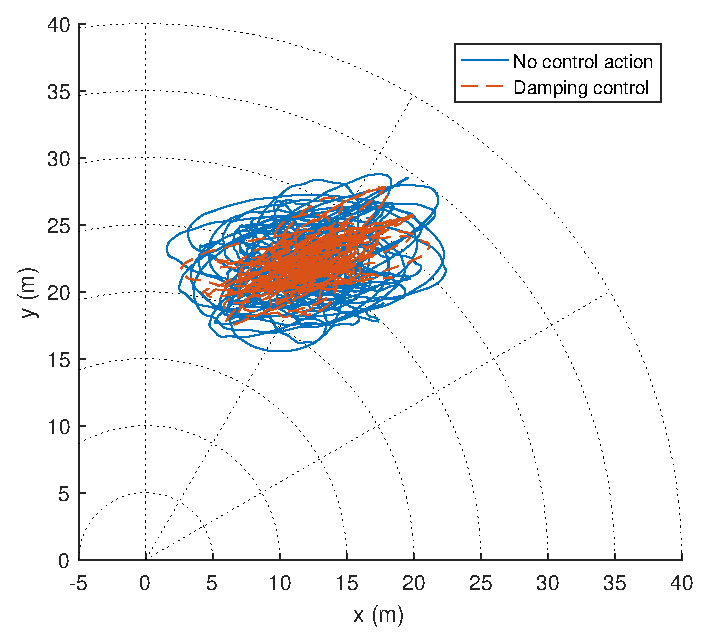
\includegraphics[width=3.0in]{Images/mooring_damping.eps}
	\caption{Platform paths under no control action and damping control mode, respectively.}
	\label{fig:mooring_damping}
\end{figure}

Fig.~\ref{fig:setpoint} depicts the performance of the platform motion when being positioned in CM2 with different fixed values of $\rho_d$.  In each simulation where the same control parameters $\vec{\Lambda}, \vec{K}_p, \vec{K}_d$ are used, the platform mainly moves along the circle arc of radius $\rho_d$, as the motions along the radial direction are constrained by the mooring lines and the setpoint control actions. When the setpoint $\rho_d > \rho_e$, the thrusters fight against the mooring system and push the platform to the radial offset $\rho_d$. As the setpoint $\rho_d$ moves closer to the field zero point when $\rho_d < \rho_e$, an increasing portion of the mean environmental loads is compensated by the thruster actions. 

\begin{figure}[htbp]
	\centering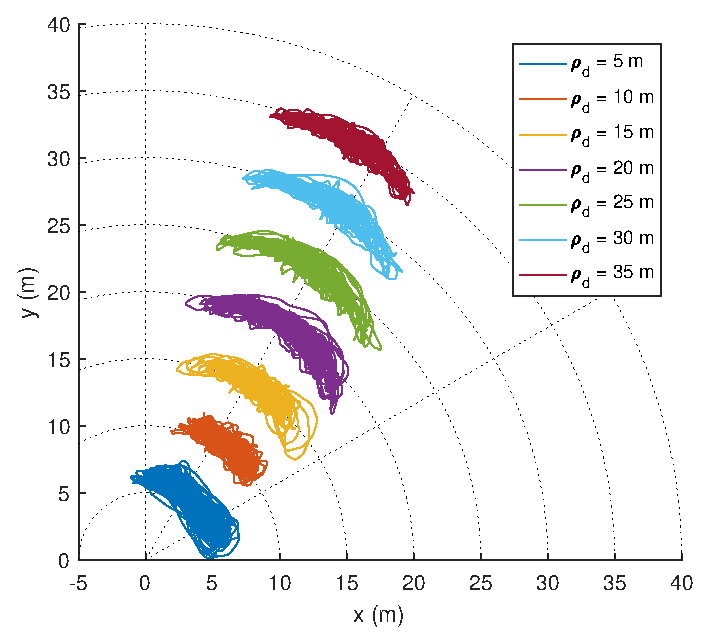
\includegraphics[width=3.0in]{Images/setpoint.eps}
	\caption{Platform paths with different radius setpoint $\rho_d$.}
	\label{fig:setpoint}
\end{figure}

Fig.~\ref{fig:power_setpoint} shows how the selection of the radius setpoint $\rho_d$ affects the power consumption level of the thrusters. The power consumed by a thruster in a DP system can be calculated by its torque multiplied by its speed of revolution \cite{arditti2015thrust}. Accordingly, the power consumption level at each radius setpoint is approximated by the mean value of $\Sigma u_i(t)^{(3/2)}$, where $u_i$ denotes the thrust force exerted by the $i$th azimuth thruster. As expected, the minima of the power consumption lies at $\rho_d = \rho_e$, where the mean environmental disturbances are mainly counteracted by the mooring system. The equilibrium position of the mooring system is considered to be the optimal setpoint for the PM system in terms of the power consumption of the thrusters. In the next section, a novel method to determine the optimal setpoint is presented for a PM system operating in an unknown environment.

\begin{figure}[htbp]
	\centering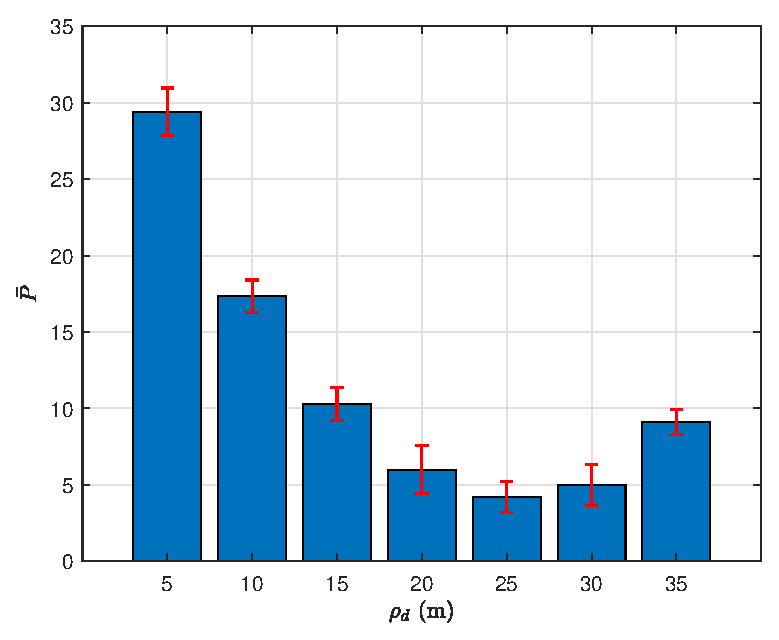
\includegraphics[width=3.0in]{Images/setpoint_power.eps}
	\caption{The mean value and standard error of the average power consumption level $\Sigma u_i(t)^{(3/2)}$ at each radius setpoint $\rho_d$ over a 5-min interval. Note that the displayed values of the vertical axis have been divided by 1000.}
	\label{fig:power_setpoint}
\end{figure}

\section{DECISION-MAKING APPROACH}
The high-level decision support for the PM control system is responsible for automatically providing the appropriate setpoints for the low-level controllers in CM2, rather than letting the operators manually decide. Maximizing the utilization of the mooring system to compensate the mean environmental loads is the primary objective of the decision-making strategy for PM systems operating in moderate sea conditions. In this section, an automated decision support agent is presented to determine the optimal setpoints, which is based on the method of reinforcement learning (RL).

\subsection{Reinforcement Learning}
A RL agent learns a state-action policy $\pi = P(a|s)$ through a Markov decision process (MDP) with observations $(s)$, actions $(a)$ and rewards $(r)$ while interacting with the environment. The final goal of RL is to select actions which maximize cumulative future reward, which can be represented by the optimal action-value function:

\begin{equation}
Q^*(s,a) = \max_\pi \mathbb{E} \left[ r_t + \gamma r_{t+1} + \gamma^2 r_{t+2} + \dots | s_t=s, a_t = a, \pi \right]
\end{equation}

\noindent where $r_t$ is the reward at time-step $t$, and $\gamma$ is the discount factor. In practice, it is common to use a linear or nonlinear function approximator to estimate the Q-function, $Q(s,a;\theta)\approx Q^*(s,a)$ \cite{sutton1999reinforcement}. In this study, the method proposed by \cite{mnih2015human-level} is adopted, which uses a feedforward neural network with weights $\theta$ as the Q-function approximator. The architecture of the neural network is illustrated in Fig.~\ref{fig:neural_network}. The state representation $s$ is the input to the neural network, and the outputs $Q(s,a)$ correspond to the approximate Q-values of the individual actions for the input state.

\begin{figure}[htbp]
	\centering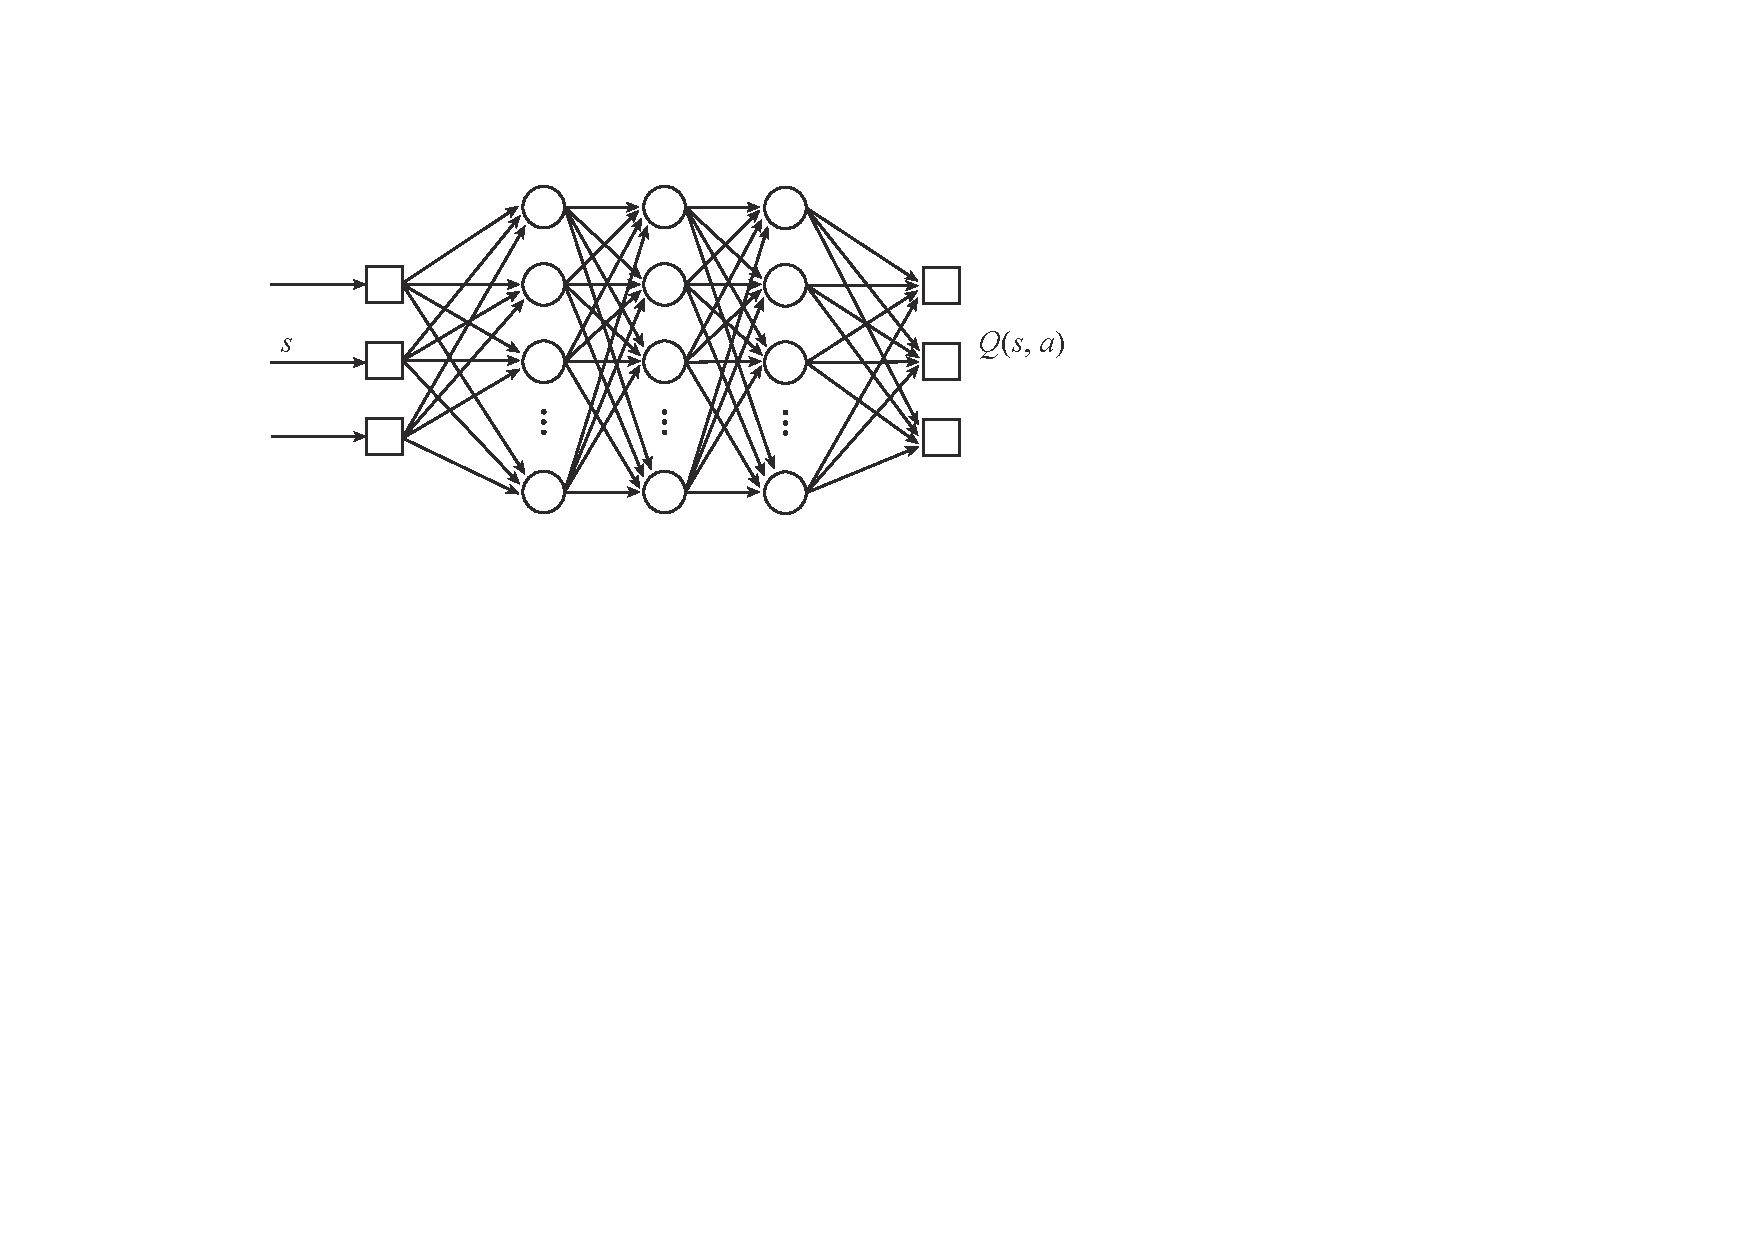
\includegraphics[width=3.0in]{Images/ann}
	\caption{Architecture of the neural network as the $Q$ function approximator.}
	\label{fig:neural_network}
\end{figure}

The training algorithm is based on Q-learning method. After taking some action $a_i$ based on an $\varepsilon$-greedy policy and observing $(s_i, a_i, r_i, s_i')$ at iteration $i$, the Q-network can be trained by adjusting the parameters $\theta_i$ to reduce the mean-squared error:

\begin{equation}
L(\theta_i) = \frac{1}{2} || Q(s_i,a_i;\theta_i) - y_i ||^2
\end{equation}

\noindent where $y_i = r_i + \gamma\max_{a'}Q(s',a';\theta_i^-)$ is the approximate target value with parameters $\theta_i^-$ from some previous iteration. The techniques of experience replay and target network are also used in the training algorithm to provide diverse and decorrelated training samples and to prevent the action selection policy from oscillating or even diverging. The samples of the RL agent's experience $(s_t, a_t, r_t, s_{t+1})$ at each time-step are stored in a replay memory, and a random minibatch is drawn from the stored samples when performing a gradient descent step on $L(\theta)$. Second, a separate network $\hat{Q}$ is used for generating the approximate targets $y_i$ in the Q-learning update. The parameters of the target network $\hat{Q}$ are replaced by the network $Q$ every $N$ updates.

The selections of optimal setpoints can be formulated as an infinite MDP. The state is the radius of the platform in the polar coordinate system. Based on the observations that the platform in CM2 always oscillates within a small range around the setpoint along the radial direction, the states can be defined by the discrete setpoints for the PM system. The actions consist of increasing or decreasing the radius setpoint by $\Delta\rho$, as well as keeping the setpoint unchanged. The set of actions can be denoted by:
\begin{equation}
\mathcal{A} = \{ 0, -\Delta\rho, \Delta\rho \}
\end{equation}
Accordingly, the states can be defined as:
\begin{equation}
\mathcal{S} = \{ \cdots, \rho_0 -2\Delta\rho, \rho_0-\Delta\rho, \rho_0, \rho_0 + \Delta\rho, \rho_0 + 2\Delta\rho, \cdots \}
\end{equation}

\noindent where $\rho_0$ is an initial selection of the radius setpoint. As a result, if the agent takes action $a$ in state $s$, we know exactly what the next state $s'$ is. Besides, the states must be within a certain range $\left(0, \rho_s\right]$, in which the upper bound $\rho_s$ is chosen to ensure the safety of the riser and mooring system. A performance measure of the PM system can be selected as the reward. Fig.~\ref{fig:power_setpoint} shows that the performance at a radius setpoint can be characterized by the power consumption level $\bar{P} = \sum \bar{u}_i(t)^{(3/2)}$ of the thrusters. Accordingly, the reward function can be defined as a mapping $r:\bar{P} \to \mathbb{R}^-$, e.g., $r(s, a) = -\bar{P}$, so that a higher power consumption level applies a heavier penalty to the given state-action pair. $\bar{P}$ is computed over the interval $\Delta t$ between two time-steps of the decision support agent. Since the environmental loads are constantly varying, the reward $r(s,a)$ is non-stationary. A trade-off must be made when choosing the time-step size $\Delta t$ of the decision support agent. On the one hand, it should be long enough for the PM system to converge to the desired radius setpoint in order to obtain a reliable reward. On the other hand, it should be as small as possible so that enough samples can be generated in a relatively short period of time to train the Q-network.

At each time-step, the model-free RL agent selects an action from $\mathcal{A}$ based on an $\varepsilon$-greedy policy that follows the greedy policy $a = \mathrm{argmax}_{a'}Q(s,a';\theta)$ with probability $1-\varepsilon$ and selects a random action with probability $\varepsilon$. Then, the new radius setpoint is sent to a first-order reference model so as to provide smooth transfer between two setpoints. A upper limit is also imposed on the rate of change of the radius setpoint, in order to ensure the stability of the low-level setpoint controller. 

\subsection{Model-based Acceleration}
In Model-free RL, the RL agent depends on sampling and observation heavily, and the inner working of the system remains unclear. On the contrary, a model-based RL has a strong advantage of being sample efficient. The reason is that a model-based RL agent can learn a world model of how the environment operates from its observations, then use the world model to train its state-action policy. In other words, the model which stores knowledge about the transitions and reward dynamics will produce a estimated next state and reward for learning a improved policy. For instance, if the agent is currently in state $s_i$, takes action $a_i$, and then observes the environment transition to state $s_{i+1}$ with reward $r_{i+1}$, that information can be used to improve its estimate of $T(s_{i+1}|s_i,a_i)$ and $R(s_i, a_i)$, which can be performed using supervised learning approaches. Once the agent has adequately modeled the environment, it can use a planning algorithm with the learned model to learn a policy\cite{silver2008sample}.

In order to build a model based RL agent, the state transition function and the reward function should be modeled at the beginning. The state-transition function can be defined as:

\begin{equation}
s_{t+1} \sim T_{\eta}(s_{i+1}|s_i,a_i)
\end{equation}
where $\eta$ is the parameter of the model. In the problem of optimal setpoint learning, the state of next time step $s_{t+1}$ is actually known and uniquely determined by $(s_t, a_t)$, since the setpoint controller of the PM system is assumed to be able to position the floating structure accurately.
On the other hand, the modeling of reward function is considerably complex, which can be written as:

\begin{equation}
r_t = {R}_{\eta}(r_t|s_t,a_t)
\end{equation}
Since the reward is calculated based on the average power consumption $\bar{P}$ in the real environment, in the planning model the power consumption needs to be accurately estimated by developing a regression model.

The construction of power consumption model is a typical supervised learning problem. The data set $\{(\rho^{(i)}_d, \bar{P}^{(i)})\}$ collected from the real world is used to from training process
to train a regression model. In this work, we use the real experience to train the regression model to estimate the average power consumption and calculate the corresponding reward value. The support vector machine (SVM) is used to establish the relation between average power consumption and radius setpoint, the radial basis function is chosen to be the kernel function of the SVM.

\begin{figure}[!htp]
	\centering
	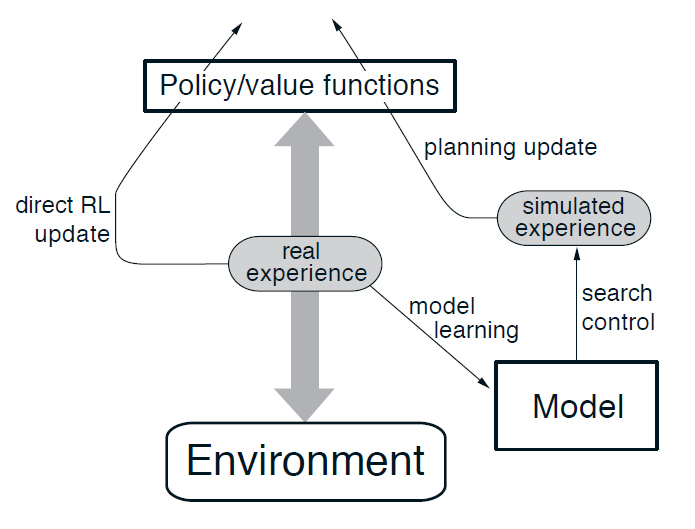
\includegraphics[width=3.5in]{Images/dyna_Q.png}
	\caption{The general model-based Architecture, which takes advantage of both real experience and simulated experience.(adapted from\cite{sutton1999reinforcement})}
	\label{fig:dyna}
\end{figure}

Fig.~\ref{fig:dyna} shows the general architecture of the model-based RL method, which is proposed by \cite{sutton1999reinforcement} . In this architecture, the training data set consists of real experience and simulated experience, and the direct model-free RL process run together with the indirect model-based RL process. At each decision time step, the model-based agent uses the trajectory $\{(\rho^{(i)}_d, \bar{P}^{(i)})\}$ of the past 3 hours to train the regression model, and it then creates a collection of simulated experience along the setpoints the agent chose in the past three hours. Also, based on the learned world model, the agent uses these data to train the Q-network together with the real experience. The additional training experience would efficiently accelerate the learning of an optimal policy.

\subsection{Simulation Results and Discussion}
The overall scheme of the intelligent PM system with model-based acceleration is given in Fig.~\ref{fig:model_based}, where the model-based decision level represents the high-level for generating the sequence of radius setpoints.
Simulations are conducted with both the high-level decision support agent and the low-level setpoint controller involved. In this study, both model-free and model-based RL agents are implemented using the Google TensorFlow framework. The Q-network has one input, one hidden layer with 20 nodes, and three outputs. ReLU activation functions are applied to the nodes in the hidden layer. We use the same network architecture and hyperparameter values of the learning algorithm (see Table~\ref{table_network}) throughout the paper. The learning rate in the table is used by the RMSProp algorithm in the gradient descent updates.

In the simulations, the time-step size $\Delta t$ of the RL agent is chosen as 5 mins, and the action step $\Delta\rho$ is 1.5$\,$m. The initial radius setpoint of the platform is 10$\,$m, and the radius setpoints must be smaller than 40$\,$m. The reward function is defined as $r(s,a) = k_0(\bar{P}-k_1)(\bar{P}-k_2)$, in which $k_0,k_1,k_2$ are carefully chosen constants.

\begin{figure}[!htp]
	\centering
	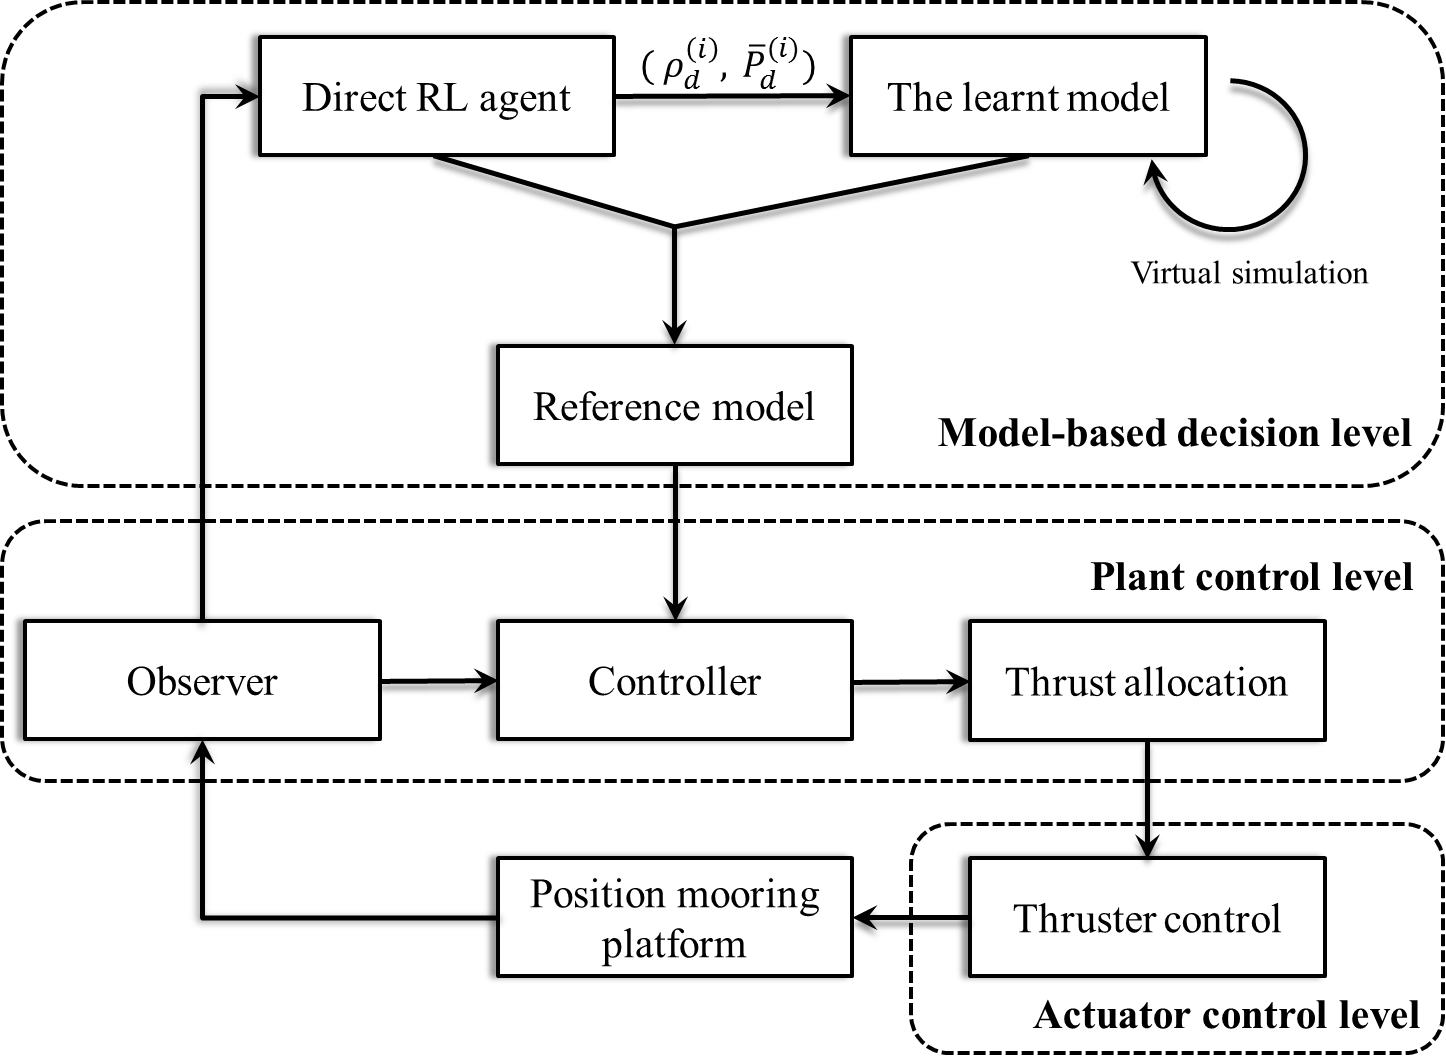
\includegraphics[width=3.3in]{Images/model_based.png}
	\caption{The overall scheme of the intellegent PM system with model-based acceleration}
	\label{fig:model_based}
\end{figure}

\begin{table}[ht!]
	\caption{Hyperparameters of the RL agent}
	\begin{center}
		\label{table_network}
		\begin{tabular}{l l}
			\hline
			Hyperparameters & Value \\
			\hline
			minibatch size & 32 \\
			replay memory size & 200 \\
			target network update frequency & 36 \\
			discount factor & 0.9 \\
			learning rate & 0.05 \\
			exploration rate & 0.1 \\
			\hline
		\end{tabular}
	\end{center}
\end{table}

\begin{table}[ht!]
	\caption{Environmental condition for simulations}
	\begin{center}
		\label{table_env_simulation}
		\begin{tabular}{c l c}
			\hline
			Type & Condition &  Heading \\
			\hline
			Wind & $U_w = 27.0$ m/s & $60^\circ \ 45^\circ \ 90^\circ$ \\
			Current & $U_c = 0.75$ m/s & $60^\circ \ 45^\circ \ 90^\circ$ \\
			Wave & $H_s = 5.27$ m, $T_p = 10.4$ s & $60^\circ \ 45^\circ \ 90^\circ$ \\
			& (Jonswap, $\gamma=3.3$) & \\
			\hline
		\end{tabular}
	\end{center}
\end{table}

\begin{figure}[!htp]
	\centering
	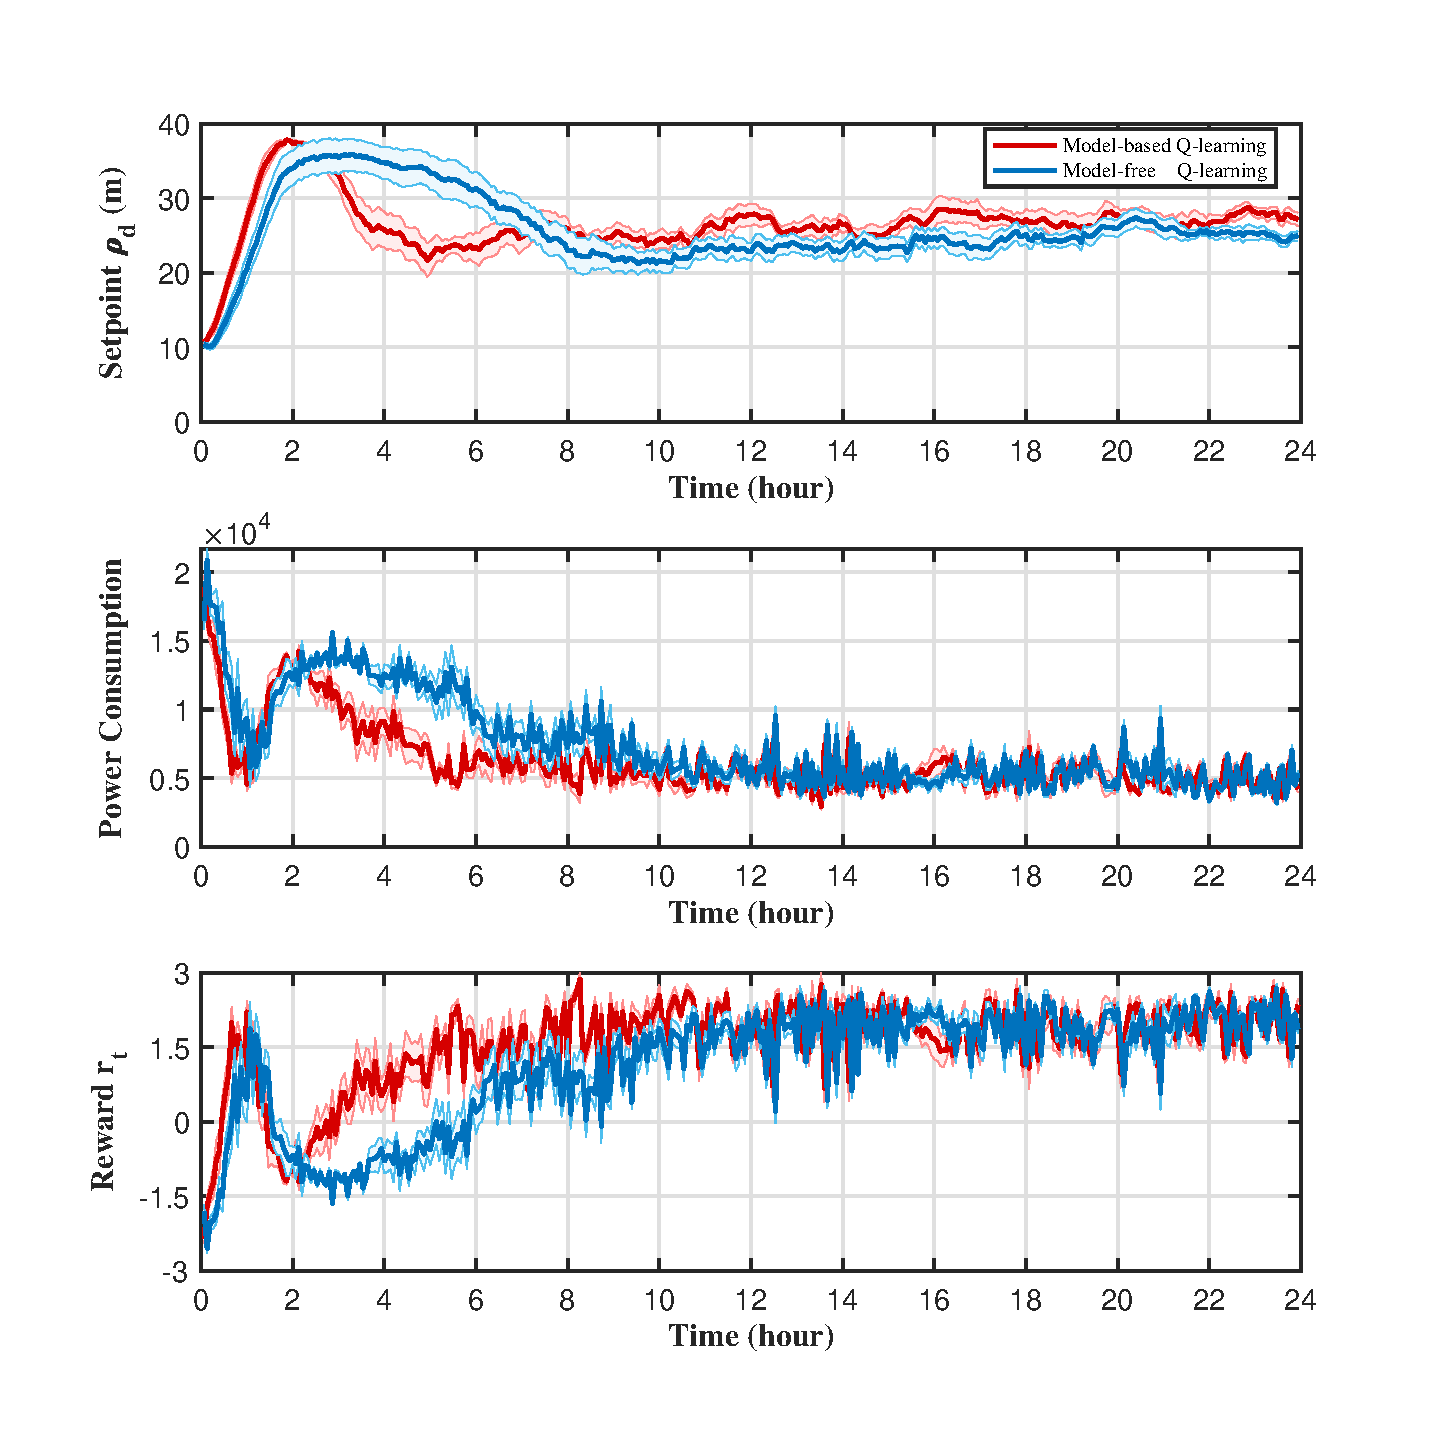
\includegraphics[width=3.5in]{Images/60_comparison.eps}
	\caption{The average setpoints $\rho_d$ determined by the RL agents, the corresponding  power consumption level and reward $r_t$ during the whole simulation, with the incident angle equals to 60 degree. The shades represent the standard errors.}
	\label{fig:rl_sim_60}
\end{figure}

\begin{figure}[!htp]
	\centering
	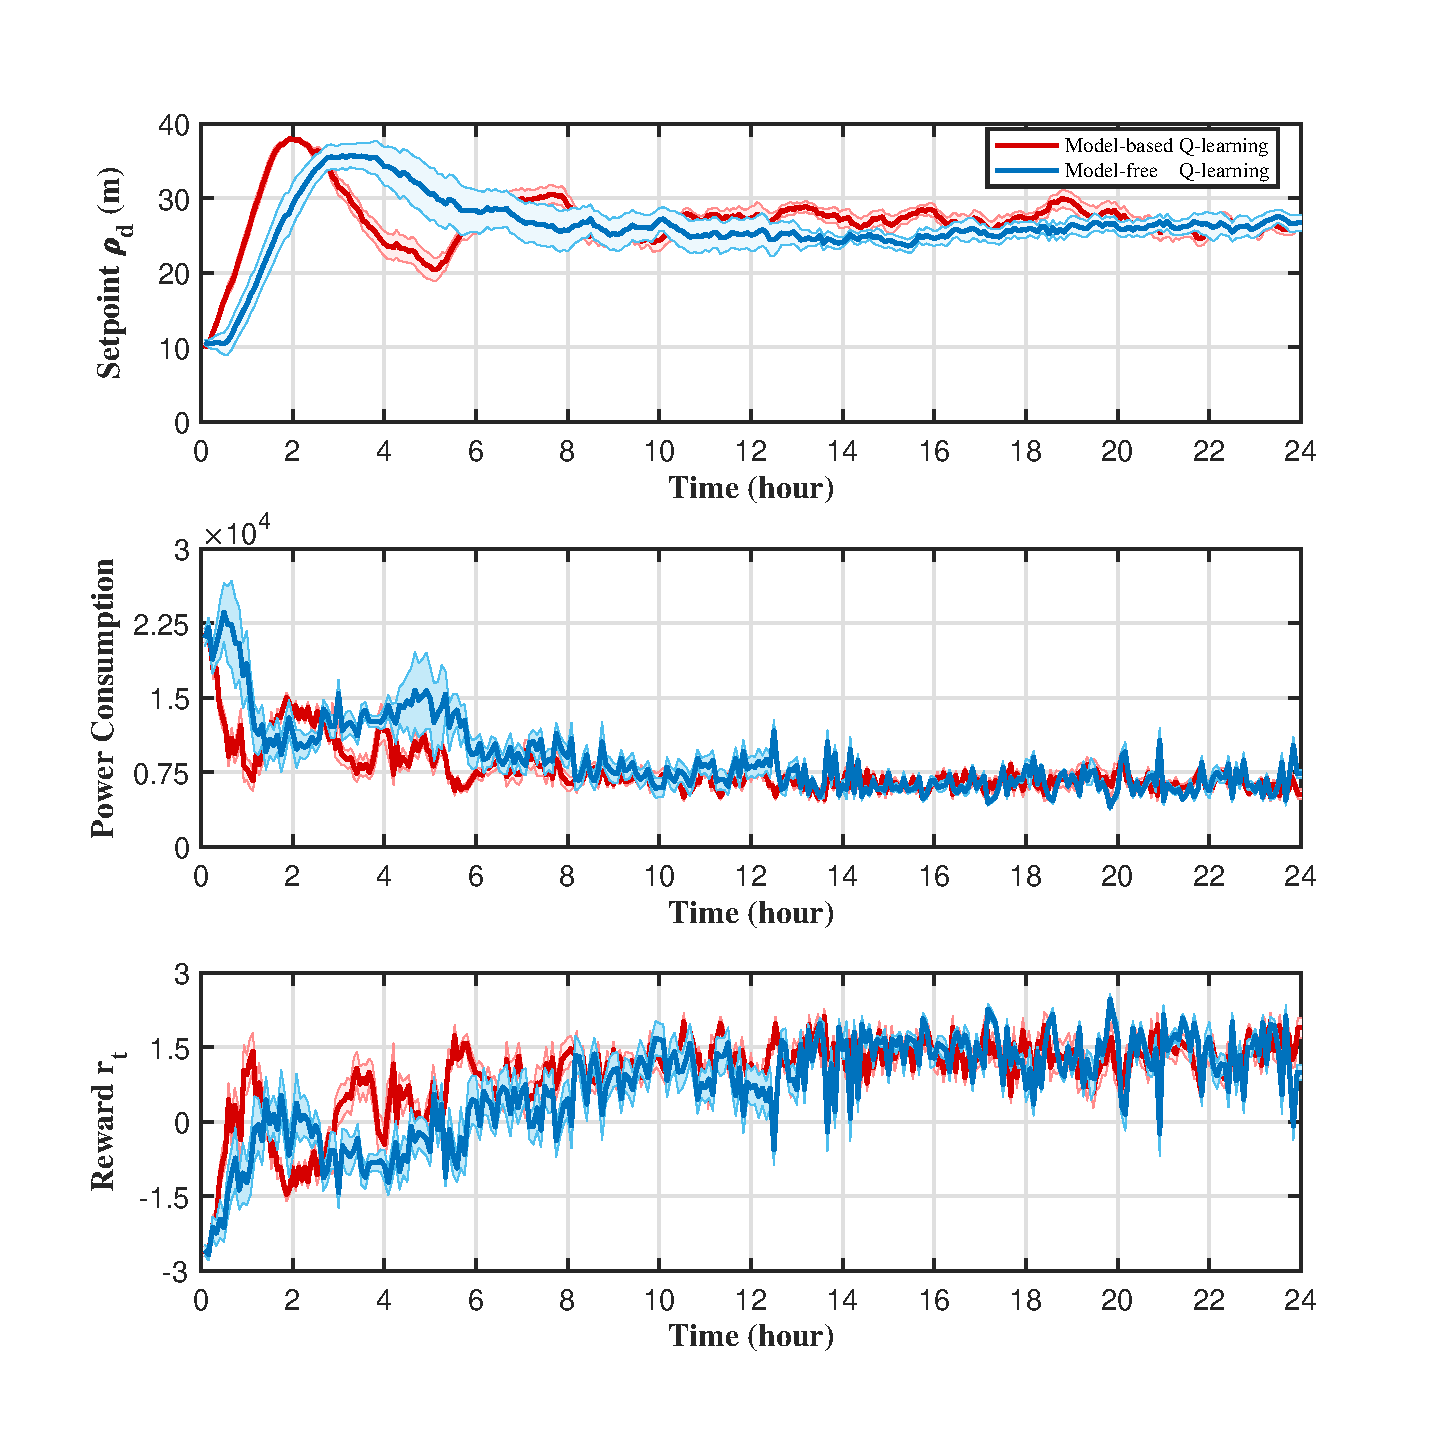
\includegraphics[width=3.5in]{Images/45_comparison.eps}
	\caption{The average setpoints $\rho_d$ determined by the RL agents, the corresponding  power consumption level and reward $r_t$ during the whole simulation, with the incident angle equals to 45 degree. The shades represent the standard errors.}
	\label{fig:rl_sim_45}
\end{figure}

\begin{figure}[!htp]
	\centering
	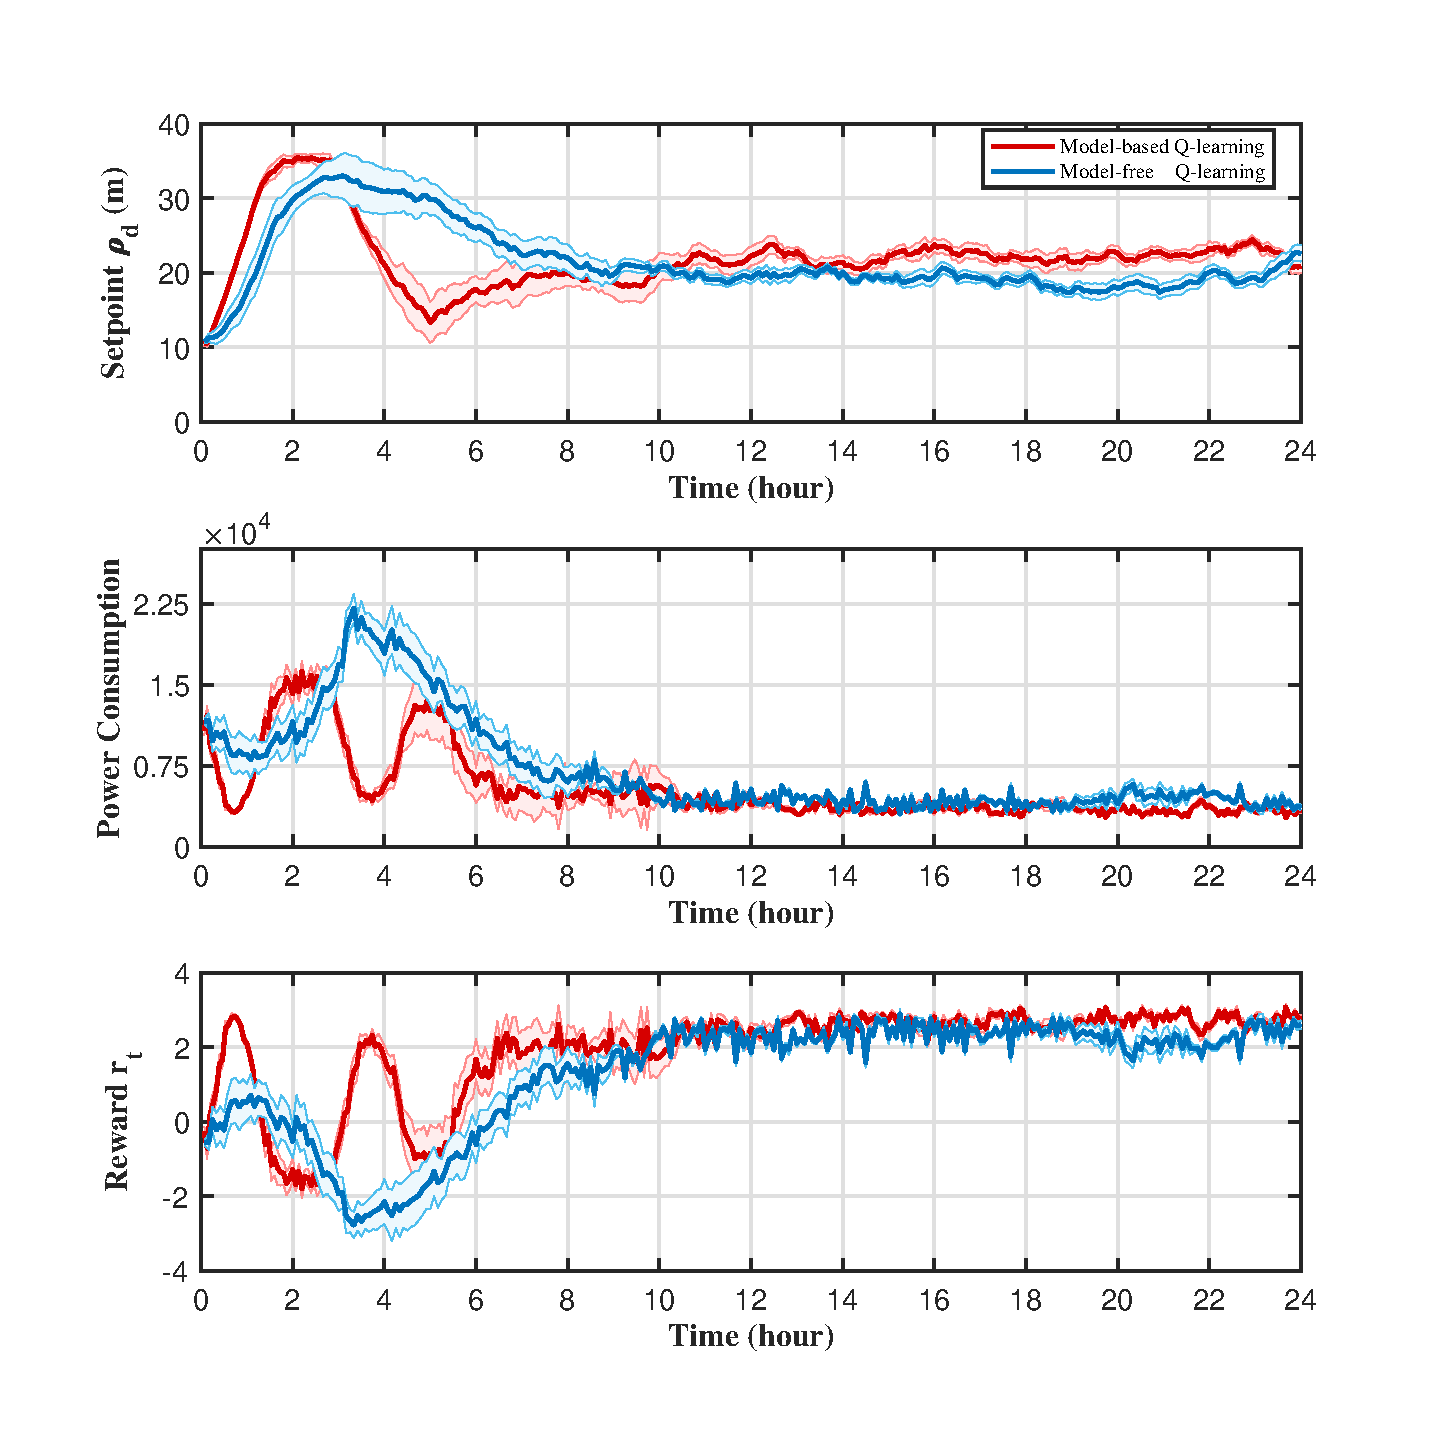
\includegraphics[width=3.5in]{Images/90_comparison.eps}
	\caption{The average setpoints $\rho_d$ determined by the RL agents, the corresponding  power consumption level and reward $r_t$ during the whole simulation, with the incident angle equals to 90 degree. The shades represent the standard errors.}
	\label{fig:rl_sim_90}
\end{figure}

Fig.~\ref{fig:rl_sim_60} illustrates the simulation results of both model-free and model-based RL agent with the incident angle equals to 60 degree. Distinct random seeds for the $\varepsilon$-greedy policy, the initial values of the Q-network parameters and selection of mini-batch are used in the 15 simulations for each RL agent. It is shown that the valley of the power consumption can be successfully found within 10 hours by the model-free RL agent, and 8 hours by the model-based RL agent. Most of the selected radius setpoints fall roughly into the range between 25.0 and 28.0$\,$m. Even though the sea condition is stationary in the simulation, the wave drift force varies continuously in each time-step. Accordingly, due to the changing environmental disturbance and the dynamics of the PM system, the reward function is non-stationary, and the radius setpoint and reward keeps fluctuating in the valley of the power consumption curve of the thrusters.

It is shown clearly that both the model-free and model-based RL approach can help the PM system find the optimal setpoint, while the later approach has a greater efficiency to reach the convergence of the optimal strategy, which may thank to the construction of the simulated experience. At the beginning of the training process, the model-free agent and the model-based agent generally generated the same radius setpoint, this is because the model-based agent can only conduct simulated experience after it collected enough state-action pair for modeling a relatively precise model, otherwise the incorrect model will negatively influence the learning process.  As mentioned before, the model-free RL relies solely on the real experience from the interaction with the environment to learn the state-action policy. Accordingly,
after the radius setpoint of the PM system moves to the upper bound for the first time, the learning process can be extremely slow, because the model-free RL agent has no experience of moving back from the upper bound at all.As a consequence, it takes quite a long time for the model-free RL agent to figure out that it is better to leave the upper bound than hanging there, in order to lower the total power consumption.

The model-free RL, however, uses simulated experience, which includes the samples of moving back from the upper bound, to train the Q-network together with the real experience. Therefore, the key to success of the model-based RL agent is the learning of the world model. Fig.~\ref{fig: start} to Fig.~\ref{fig: end} show how regression model of power consumption is built over time. The red dots represent the real average power consumption data at each experienced setpoint radius for the last three hours, and the blue curve is the fitted curve by the support vector machine. It can be seen that the support vector machine with the radial basis function as the kernel function can fit the data points quite well. It can not only generate reliable simulated experience in the local areas, but also demonstrate certain generalization capabilities in predicting
the power consumption in a global manner. Therefore, the model-based agent reaches the optimal position quicker than the model-free agent.

On top of that, further numerical experiments with different environment conditions were taken to validate the robustness of the proposed scheme (see Table~\ref{table_env_simulation}). Fig.~\ref{fig:rl_sim_45} and Fig.~\ref{fig:rl_sim_90} gives the simulation results with different environment incident angles. Under both situations, the model-free and model-based agent successfully found the optimal radius setpoint region within 10 and 8 hours respectively. A larger fluctuation happened when the incident angle is $45^\circ$, the optimal radius setopint region under such environment condition is between 26m and 28m. On the other hand, when the incident angle is $90^\circ$, the floating structure reached a steady setpoint radius(between 20 and 22m) with a relatively stable power consumption level and a better reward after a quick exploration in first six hours. 

Compared with $60^\circ$ and $90^\circ$ case, the simulation with a $45^\circ$ heading direction experienced a larger power consumption fluctuation,  this is because the external environment force is asymmetrically applied to the floating structure, resulting an uneven force sharing for thrusters and mooring lines. As mentioned before, the accuracy of the model has great impact on the model-based reinforcement learning. In $45^\circ$ heading direction case, the same decided radius setpoint may get different power consumption level at different times, which might negatively influence the model-based learning process. 

Overall, the simulation results demonstrate that the RL agent based on both model-based and model-free approach is fairly effective in finding the optimal radius setpoints for the PM system on the basis of the continuous decreasing trend of the power consumption level during the training process, and the model-based approach is shown to increase the learning speed of the RL agent.


\begin{figure}[!htp]
	\centering
	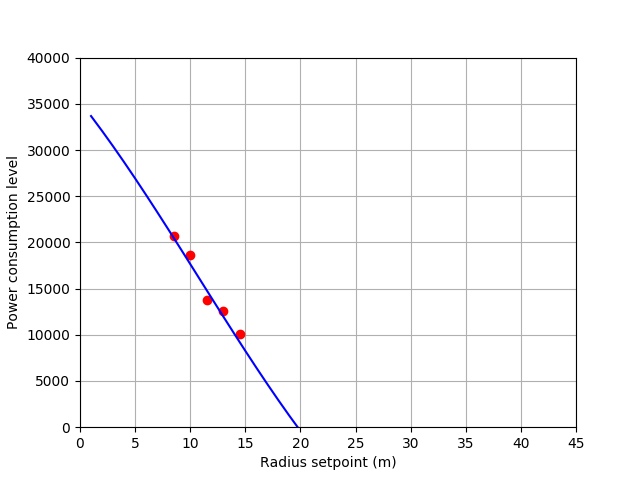
\includegraphics[width=3in]{Images/reward_004.png}
	\caption{The learned model of power consumption when $t$ = 25 min.}
	\label{fig: start}
\end{figure}

\begin{figure}[!htp]
	\centering
	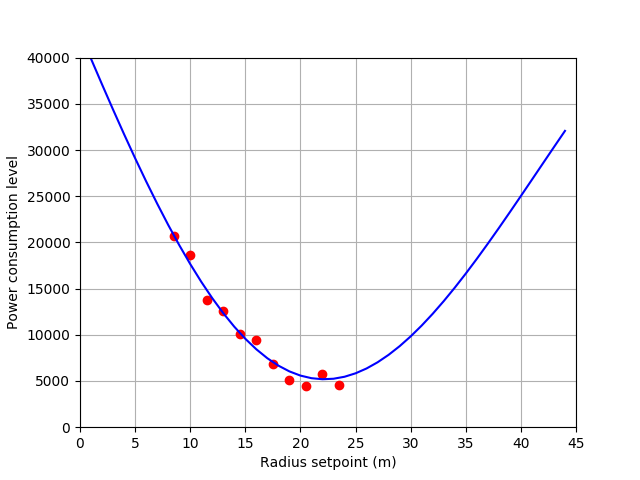
\includegraphics[width=3in]{Images/reward_010.png}
	\caption{The learned model of power consumption when $t$ = 55 min.}
\end{figure}

\begin{figure}[!htp]
	\centering
	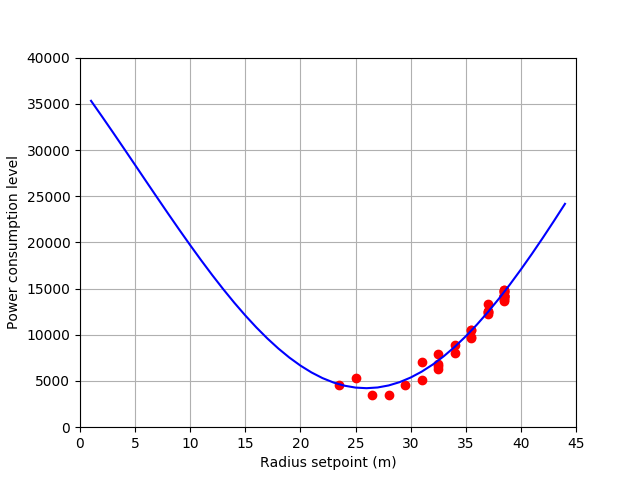
\includegraphics[width=3in]{Images/reward_045.png}
	\caption{The learned model of power consumption when $t$ = 230 min.}
\end{figure}

\begin{figure}[!htp]
	\centering
	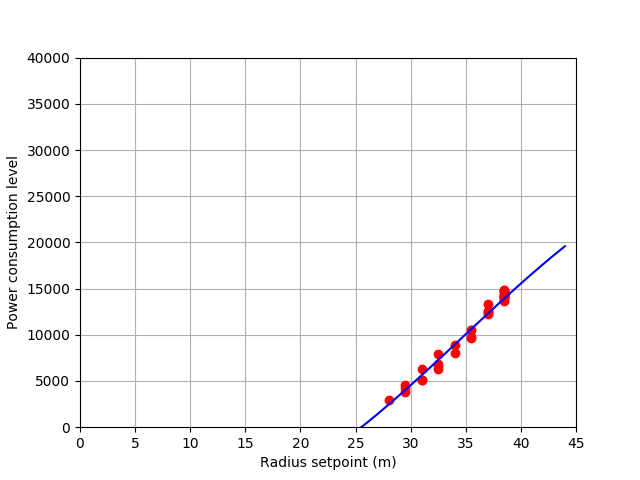
\includegraphics[width=3in]{Images/reward_051.png}
	\caption{The learned model of power consumption when $t$ = 260 min.}
\end{figure}

\begin{figure}[!htp]
	\centering
	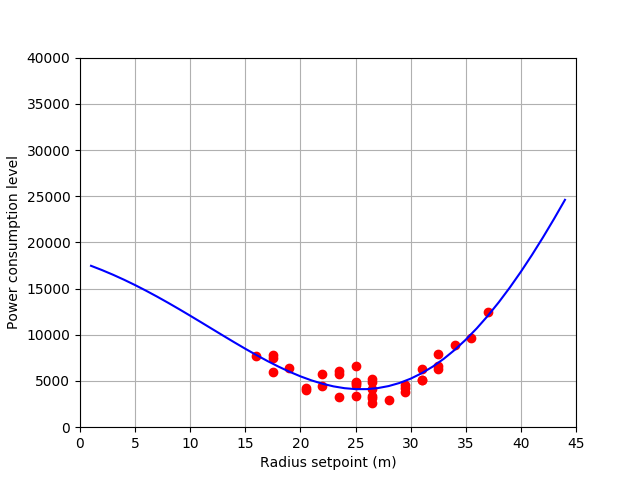
\includegraphics[width=3in]{Images/reward_074.png}
	\caption{The learned model of power consumption when $t$ = 375 min.}
\end{figure}

\begin{figure}[!htp]
	\centering
	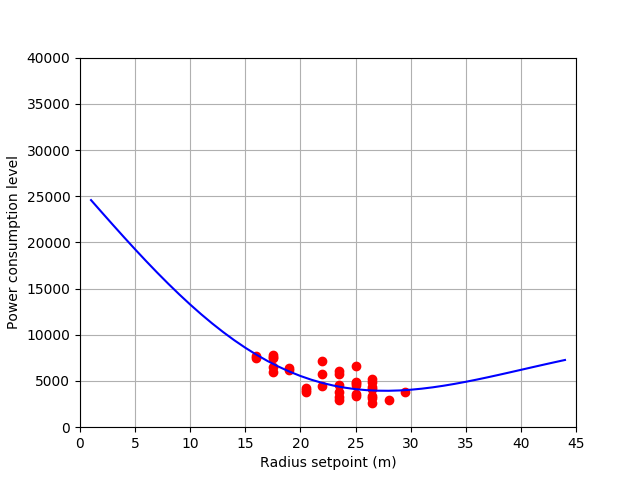
\includegraphics[width=3in]{Images/reward_085.png}
	\caption{The learned model of power consumption when $t$ = 430 min.}
	\label{fig: end}
\end{figure}


\section{CONCLUSIONS}
In this paper, a novel decision-making strategy for selecting optimal setpoints is developed for PM systems operating in moderate sea conditions. Based on simulation results, it is shown that the equilibrium position of the mooring system is the optimal setpoint to follow, which can reduce the power consumption of the thrusters and maximize the utilization of the mooring lines. 

The optimal setpoints are determined by the proposed intelligent decision support agent based on both model-free and model-based reinforcement learning, in which neural networks are used to approximate the action-value functions of the learning algorithm. The simulation results demonstrate that for a given unknown stochastic sea condition,the RL agents can successfully find the desired setpoints through extensive interactions with the environment, while the model-based approach can profoundly accelerate the learning speed of the agent, showing its promising potential in future applications.

In the future, it will be important to conduct model tests for further validation. Moreover, the proposed method will be implemented for a non-collinear unsteady ocean environment, and the case of damaged mooring line will be studied as well, in order to further validate the capabilities of the intelligent decision-making agent in more realistic environments.


\begin{acknowledgements}
The authors greatly acknowledge the support of the China Postdoctoral Science Foundation  (Grant No. 2017M621479), the Open Foundation of State Key Laboratory of Ocean Engineering (Grant No. 1717) and the 7th Generation Ultra Deep Water Drilling Unit Innovation Project.
\end{acknowledgements}

% BibTeX users please use one of
\bibliographystyle{spbasic-unsort}      % basic style, author-year citations
%\bibliographystyle{spmpsci}      % mathematics and physical sciences
%\bibliographystyle{spphys}       % APS-like style for physics
\bibliography{refs}   % name your BibTeX data base
\end{sloppypar}
\end{document}
% end of file template.tex